%\documentclass[german,bachelor]{webisthesis}
\documentclass[english,master]{webisthesis}
% When you change the language, pdflatex may halt on recompilation.
% Just hit enter to continue and recompile again. This should fix it.

%
% Values
% ------
\ThesisSetTitle{Supporting the Discovery of Energy Hot-Spots via Performance Alignment}
\ThesisSetKeywords{These, Are, My keywords} % only for PDF meta attributes

\ThesisSetAuthor{Max Weber}
\ThesisSetStudentNumber{110068}
\ThesisSetDateOfBirth{04}{05}{1991}
\ThesisSetPlaceOfBirth{Jena}

\ThesisSetSupervisors{Prof.\ Dr.\ Ing.\ Norbert Siegmund,Prof.\ Dr.\ Unknown Yet}

\ThesisSetSubmissionDate{20}{5}{2018}

%
% Suggested Packages
% ------------------
\usepackage[numbers,square]{natbib}

%   Allows citing in different ways (e.g., only the authors if you use the
%   citation again within a short time).
%
\usepackage{booktabs}
%    For tables ``looking the right way''.
%
%\usepackage{tabularx}
%    Enables tables with columns that automatically fill the page width.
%
%\usepackage[ruled,algochapter]{algorithm2e}
%    A package for pseudo code algorithms.
%
%\usepackage{amsmath}
%    For tabular-style formatting of mathematical environments.
%

% Create links in the pdf document
% Hyperref has some incompatibilities with other packages
% Some other packages must be loaded before, some after hyperref
% Additional options to the hyperref package can be provided in the braces []
\usehyperref[backref] % This will add back references in the bibliography

\RequirePackage{xcolor}
\newcommand{\todo}[1]{\colorbox{red}{\color{white}\sffamily TODO: #1}}
\newcommand{\featureit}[0]{\textit{feature}}
\newcommand{\featuresit}[0]{\textit{features}}
\newcommand{\fmit}[0]{\textit{feature model}}
\newcommand{\fmsit}[0]{\textit{feature models}}

\begin{document}
\begin{frontmatter}
  \begin{abstract}
During the past years the information and communication technologies (ICT) sector grew exponentially. It is to be expected that this trend continues in the next years. Currently, the energy needed to supply data centers, servers and every kind of computational device increases with the progress of the ICT sector. This poses economic and environmental complications.\\
To have energy available it has to be generated, stored and delivered. Storage requires materials for batteries, delivery requires infrastructure and also a big issue in this context is cooling down the hardware. For years, economy tries to save energy consumption of hardware (e.g. European Union energy label). But while hardware primarily consumes energy, it can only be as efficient as the software that operates that hardware.\\
This master thesis proposes and implements a tool to analyze software regarding their energy consumption. In relation to other research in this area, this thesis tries to answer the following questions. Is it possible to identify energy leaks in software? Does configuration of software affect energy consumption? Is it possible to predict energy consumption of software with unknown configurations? And finally, does visualization of energy hot spots in source code help programmers to rectify them?\\
To answer this questions we want to analyze performance and energy consumption of software projects written in Java. We want to profile the project on the one hand with different configurations to identify configuration sensitivity and on the other hand with different inputs to identify input sensitive parts. Next, we want to relate performance to the energy consumption. After that we want to investigate up to which level it is possible to predict energy consumption and performance of untested configurations. \\
Finally, we want to validate our work by showing that our approach can automatically detect and rank energy leaks in software projects for which such leaks are known. To verify that out tool helps software developer to rectify energy hot spots in source code we will conduct a user study with and without help of the tool.\\
If our results are satisfying we have created a tool which helps software developer to be aware of their of their energy footprint. So there will be more energy efficient programs that will have less energy costs.
  \end{abstract}

  \tableofcontents

  %\chapter*{Acknowledgements} % optional
  %I thank the authors of the webisthesis template for their excellent work!

  %\listoffigures % optional

  %\listoftables % optional

  %\listofalgorithms % optional
  %    requires package algorithm2e

  % optional: list of symbols/notation (e.g., using the nomencl package)
\end{frontmatter}

% ---------------------------------------------------------
% Main content
% ---------------------------------------------------------

\pagenumbering{arabic}
%\onehalfspacing
% ---------------------------------------------------------
\chapter{Introduction}
\label{chap:introduction}
% ---------------------------------------------------------

Since the beginning of software engineering, developers try to produce software which performs good. 
Over the years, software has to run more difficult, complex and computing-intensive tasks. 
Used Hardware, software and technology becomes more and more complex.
Every time software has to fulfil different quality properties depending on the domain or use case. 
This includes aspects like reliability, security, maintainability and performance. 
Each aspect is analyzed and described in several publications. 
The analysis of reliability aims at the reduction and prevention of application problems that effect users.
Also, security and maintainability have been subjects of research for decades~\cite{liskov1972design,johnstone1978computer,yau1980some}. 
The efficiency aspect of software systems describes how source code and software architecture perform in run-time scenarios. 
Performance has always been among the most important aspects.

In this thesis we analyze performance of software. 
There exist different definitions of performance regarding software and software systems. 
While performance from an end user's perspective describes the ability that users can perform a certain task without perceivable delay or without irritation, the developers perspective is explained by so called non-functional properties~\cite{Molyneaux:2009:AAP:1550832}.
These properties provide a way to judge the quality of software systems. 
This was already done by other researchers~\cite{Molyneaux:2009:AAP:1550832,weber2005key,siegmund2015performance,smith1993software}. 
This work differs from others in that we analyze the performance of software projects on method level, which cause different challenges (described in chapter~\ref{perf_measure}). 
We refer to identification of performance problems on a method level as \textit{performance hot-spots}.

Nowadays, almost every software system can be configured by numerous options. 
This configurability provide the possibility to customize program's behaviours for users needs. 
For example, databases typically let users configure options like encryption, compression, cash size and many others. 
While this flexibility helps to make software customizable to the user, it also causes an increased effort during testing, maintaining and analysis of performance. 
Not only the size of the configuration space is hard to grasp by users; but also possible constraints among options make configuring a software systems problematic.
Because programs with more than 217 simple binary configuration options provide more different configurations possibilities than atoms in the universe~\citep{krueger2006new}, which make testing and analysing them all impracticable. 
Note that there are software projects with much more options to configure them. 
This high configurability leads users to pick default configurations instead of configurations which let the system perform as desired. 
Therefore, we will sample configurations to get an subset which describes the whole configuration space for our analysis, so we do not have to analyze them all.

% roughly describe way to detect performance hot spots on function level
% specialization of this work
% ------------GOAL---------------- 
Our goal is to analyze performance and model the influence of configuration options of software systems. 
To understand the influence of configuration options, we profile each subject system with an appropriate profiler to extract the runtime of single functions of the running program. 
We decided to take Java projects for our subject systems, so we also want to analyze the influence of the environment in which the tests are running. 
A visualization of our results directly in the source code within an \ac{IDE} will help developers identify possible performance hot-spots. 
An overview of the performance distribution over all functions in a project gives new perspectives to support performance analysis.

% ------------Approach----------------

To analyze \textit{performance} we follow a five step approach:

\begin{enumerate}
	\item Identification of whole configuration spaces and determining different workload levels.
	\item Profiling the execution of software projects with sampled configurations and different workloads.
	\item Processing extracted data to assess performance on function level and to determine significance of the data.
	\item Model the influence of configuration options to performance.
	\item Learning influence of configurations on functions of the software.
	\item Visualize performance hot-spots directly in the source code and create suitable visualizations of performance dependencies.
\end{enumerate}


% ------------Contribution------------

Our work has the following contributions.
First, we give some background knowledge and provide an overview of related work in chapter~\ref{b_rel_work}.
In section~\ref{perf_measure}, we provide an analysis of available Java profilers.
Then, we model the subject systems as feature models to define the space of all valid configurations in section~\ref{case_studies} and in appendix~\ref{feature_diagrams}. 
Next, we provide a detailed analysis of the influence of performance on the environment on which the software runs in section~\ref{discussion}. 
We also compare different sampling strategies to evaluate coverage of the configuration space in section~\ref{perf_measure_sampling}. 
%Then we analyze the learnability of performance on method level influenced by configurations in section~\ref{learnability}. 
Furthermore, we provide an overview visualization of the influence of configurations on performance in section~\ref{flame_graph}. 
Finally, we developed an Eclipse plug-in to visualize performance hot-spots directly in the \ac{IDE} in section~\ref{eclipse_plugin}.
% direct in source code 
% provide an overview of performance of configurable software systems

% Analyze performance and energy consumption of Software Projects written is JAVA.
% Analyze performance on function level
% Vary projects configuration to identify configuration sensitivity
% Vary projects input to identify input sensitive parts
% Relate energy consumption of the system to parts of the software
% Predict energy consumption and performance of untested configurations


% ---------------------------------------------------------
\chapter{Related Work}
\label{rel_work}
% ---------------------------------------------------------

\section{Paper}

A Survey about Performance Evaluation of Component-based Software Systems \cite{koziolek2010performance}.

Cycle-accurate simulation of energy consumption in embedded systems. Comparison between performance and energy computed by their simulator \cite{simunic1999cycle}.

Report on experience in using the Running Average Power Limit (RAPL) energy sensors available in recent Intel CPUs for measuring energy consumption
of short code paths \cite{hahnel2012measuring}.

Early Performance Testing of Distributed Software Applications \cite{denaro2004early}.

Green Tracker measurement tool (for estimating the
energy consumption of software)\cite{amsel2010green}.

Software performance engineering \cite{smith1993software}.

The Future of Software Performance Engineering \cite{woodside2007future}.


% ---------------------------------------------------------
\chapter{Big Picture}
\label{chap:method}
% ---------------------------------------------------------
This chaper super intro because importantst chapter


\section{Process}

Goal: we need software to test the performance 

Defining: of configuration options of the software
workload of the software

profile software execution \ref{perf_measure}
choose appropriate sampling strategie
repeate execution number sample times

because software runs on real hardware measurements might be biased
extract execution bias (external mesurement impact)

if bias is acceptable use data to learm variability model of software 

if it is acceptable calculate model for each function (WHY?)
showing influences of configuration options to each function

Visualisation plugin eclipse to mark possible hot-spots direct in IDE

Flame Graph as overview distribution of functions



Our Workflow:

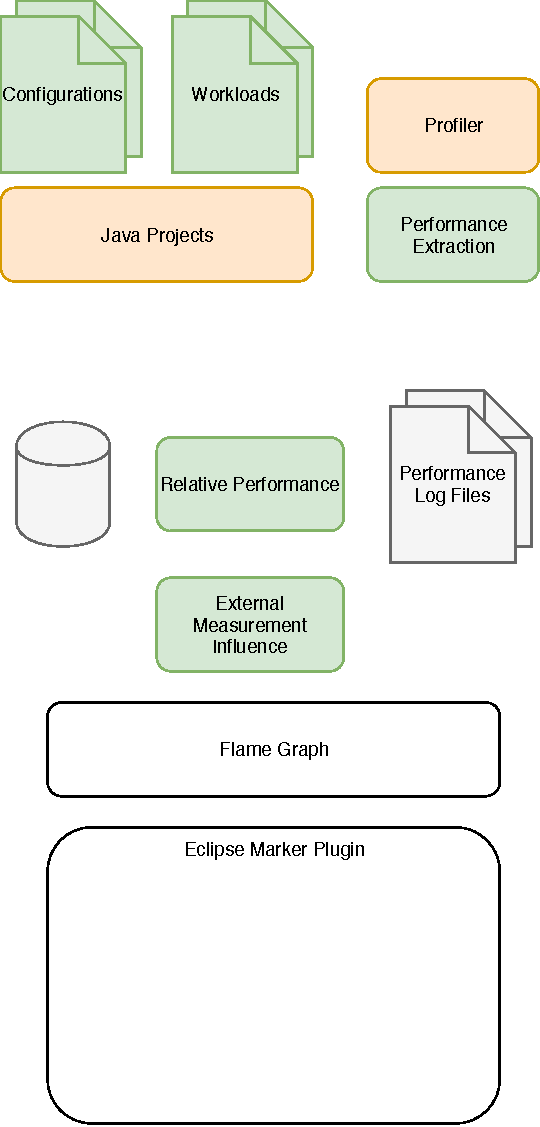
\includegraphics[width=0.6\textwidth]{images/Workflow}

\section{Case Studies}
\label{case_studies}

Eingrenzung auf Java software because, widespread, popular, often used, runs on billions of devices

% 3 Java projects 
% 3 different kinds of projects to depict variety
% Configurable, Workload of projects to manage execution time and to validate results of projects with different workloads
% different configuration space 
% different ammount of configuration options
% 

\subsection{Catena}

 Project description
% Project size in Classes and Functions
% Project properties (SPL Model)
% Features explained
% Workload

\subsection{H2}

Project description
% Project size in Classes and Functions
% Project properties (SPL Model)
% Features explained
% Workload

\subsection{Sunflow}

Project description
% Project size in Classes and Functions
% Project properties (SPL Model)
% Features explained
% Workload

\section{Sampling}
\label{perf_measure_sampling}

Why sampling?
Configuration space 
Course of high dim spaces
Random Sampling

\subsection{Binary Sampling}

\subsubsection{Option-Wise}

\subsubsection{Negative-Option-Wise}

\subsubsection{t-Wise}

\subsubsection{Binary-Random}


% Why random ... other paper.

\subsection{Numeric Sampling}

\subsubsection{One Factor at a Time}

\subsubsection{Central Composite}

\subsubsection{Placket-Burman Design}

% other strats
% Distance computation

\section{Monitoring/Profiling}
pitfalls
strategies 
solutins
expected outcome

% ---------------------------------------------------------
\chapter{Performance Measurement and Lernability}
\label{chap:p_measurement}
% ---------------------------------------------------------

 Measurement of performance is an important aspect of all kinds of science. 
% performance measurement of java 
% performance term is explained in chap Background
% how does mesurement of performance work in general?
% Impact from OS and Hardware (CPU overclock, memory access, memory level)
% Sampling Strategies


\section{Java Performance Mesurement}
\label{perf_measure}

Java specific impacts on program execution 
% Related paper 
% Garbage collector
% Java Byte code optimization

\subsection{Java Performance Measurement Tools}

Because of the thing that it is importatant to know how well your program performs many different tools arose in the area of performance measurement. Some of them are developt for specific requirements others are restricted in different ways. In the following part of work there will be a summary of all important measurement tools for Java programs.


\subsubsection{\href{https://profiler.netbeans.org/}{HPROF}}

%The Java 2 Platform Standard Edition (J2SE) has always provided a simple command line profiling tool called HPROF for heap and cpu profiling. HPROF is actually a JVM native agent library which is dynamically loaded through a command line option, at JVM startup, and becomes part of the JVM process. By supplying HPROF options at startup, users can request various types of heap and/or cpu profiling features from HPROF. The data generated can be in textual or binary format, and can be used to track down and isolate performance problems involving memory usage and inefficient code. The binary format file from HPROF can be used with tools such as jhat to browse the allocated objects in the heap.

%In J2SE Version 5.0, HPROF has been implemented on the new Java Virtual Machine Tool Interface. 


\subsubsection{\href{https://profiler.netbeans.org/}{NetBeans Profiler}}

%NetBeans profiler is a fully featured Java profiling tool integrated into the NetBeans IDE. The features include CPU, memory, threads, locks and SQL queries profiling as well as basic JVM monitoring, allowing developers to be more productive in solving performance and memory issues.


\subsubsection{\href{https://www.ej-technologies.com/products/jprofiler/overview.html}{JProfiler}}

%JProfiler is a commercially licensed Java profiling tool developed by ej-technologies GmbH, and is mainly designed for use with Java EE and Java SE applications. It combines CPU, Memory and Thread profiling into one application and is useful for developers as it can be used to analyze performance bottlenecks, memory leaks, CPU loads  and resolve threading issues and supports local profiling (analysis of applications that are running on the same machine on which the JProfiler software is installed) and remote profiling (this is where it allows for the analysis of Java applications which are running on remote machines which JProfiler software is not installed on.).


\subsubsection{\href{http://visualvm.github.io/}{VisualVM}}


%VisualVM is a tool derived from the NetBeans platform and its architecture is modular in design meaning its easy to extend through the use of plugins.

%Visual VM allows you to get detailed information about your Java applications while they are running on a Java Virtual Machine (JVM). Data generated can be generated and retrieved by the Java Development Kit (JDK) tools and all the data and information on multiple Java Applications can be viewed quickly both local and remote running applications.  It is possible to also save and capture the data about the JVM software and save the data to the local system, and then view the data later or share it with others.

%Visual VM can do CPU Profiling, memory Profiling, run garbage collections, take snapshots and more.


\subsubsection{\href{http://patty.sourceforge.net/}{Java Performance Analysis Tool (Patty)}}

%The ``Patty'' project is aimed at providing a profiling tool for the Java 1.5.0 and higher Virtual Machines only (depending on backwards compatibility in JVMTI interface ). The difference with other profilers is this project maintains a very high emphasis on targeted profiling and allows users to switch profiling features on and off at runtime.


\subsubsection{\href{http://jiprof.sourceforge.net/}{Java Interactive Profiler}}

%JIP is a code profiling tool. It allows you to turn the profiler on and off while the JVM is running. JIP is pure Java. It takes advantage of the Java5™ feature which allows you to hook the classloader. JIP adds aspects to every method of every class that you want to profile. These aspects allow it to capture performance data. JIP actually tracks the amount of time used to gather performance data and factors that time out of its analysis. Filters by package/class name.


\subsubsection{\href{http://profiler4j.sourceforge.net/}{Profiler4J}}

%Profiler4j is a dedicated CPU profiler Java that is user friendly and supports remote profiling and can be configured “on the fly”. Notable features include that its based on dynamic bytecode instrumentation, it as no native library nor requires an executable. Further notable features are that its done 100\% in Java, can provide graphical information with a call graph, call tree, memory monitor, and class list. and supports fine-grained configuration. It is currently released under the Apache License v2.0.


\subsubsection{\href{http://jrat.sourceforge.net/}{JRat}}

%The Java Runtime Analysis Toolkit is a low overhead, easy to use, open source performance profiler for the Java platform. JRat monitors an application's execution and persists performance measurements. This data can then be viewed and analyzed using the JRat Desktop, a Swing application.


\subsubsection{\href{http://ejp.sourceforge.net/}{Extensible Java Profiler}}

%Extensible Java Profiler (EJP) is an open-source profiling tool for Java with a scalable and extensible architecture, allowing its usage for exotic programming languages that use a Java backend.

%EJP is based on the Java Virtual Machine Profiler Interface (JVMPI). On the contrary of Sun's hprof tool, which generates statistical information, it logs every single method invocation. It can be used to trace the execution of small parts of Java programs and display it in hierarchical trees with some elements hidden or highlighted.


\subsubsection{\href{http://www.khelekore.org/jmp/}{JMP - Java Memory Profiler}}

%JMP is a profiler for java that can be used to trace objects usage and method timings. Since jmp use jvmpi it only works with java/1.2 up to java/1.5. Work has started on tijmp, a new profiler that uses the the tools interface (jvmti). JMP normally uses one window to show the classes in memory. Each class has summary information for number of instances and total bytes of used memory for all the instances. JMP can perform heap analysis and has the ability to show which objects own (have references to) all the objects of a specified class. This is a great way to find memory leaks. JMP also shows method timings and calls in another window. Several columns show time taken in the method, number of calls to each method, time taken in methods called. 
%JMP collects information about which method are called and from where, this information is used to build call graphs. JMP interacts with the normal java threads and also uses one extra thread for GTK+ with a timer to systematically update the stats. JMP is written in C, it is designed for speed. 


\subsubsection{\href{http://www.khelekore.org/jmp/tijmp/}{TIJMP - Tools Interface Java Memory Profiler}}

%TIJmp is a memory profiler for java. TIJmp is made for java/6 and later. TIJmp is written to be fast and have a small footprint, both memory- and cpu-wise. This means that the jvm will run at almost full speed, until you use tijmp to find some information. TIJjmp uses C code to talk to the jvm and it uses swing to show the the tables of information. So tijmp is written in C (using jvmti and jni) and Java. TIJmp runs in the same jvm as the program being profiled. This means that it can easily get access to all things jvmti/jni has to offer.


\subsubsection{\href{https://sourceforge.net/projects/jmeasurement2/}{JMeasurement}}

%JMeasurement is a free and simple java api for monitoring runtime and usage (count, parallel activation, last activation) of user defined points in java production code. It is simple to use and extended. JMX is supported. Actual version is always in maven central.


\subsubsection{\href{http://homepages.mcs.vuw.ac.nz/~djp/djprof/}{DJProf}}

%DJProf is an experimental tool for profiling Java programs which employs AspectJ to insert the necessary instrumentation for profiling rather than, for example, the Java Machine Profiler Interface (JVMPI). DJProf can be used to profile Java programs without modification (i.e. there is no need to recompile them for profiling) and does not require the user to have any knowledge of AspectJ.


\subsubsection{\href{https://github.com/joachimhs/Montric}{EurekaJ -> Montric}}

%EurekaJ is an Open Source, Standards based profiler tool for Java applications. EurekaJ integrates with the Java agent BTrace. BTrace has a large feature set that goes hand in hand with features for EurekaJ. Motric 1.0 is the further developed version of EurekaJ.


\subsubsection{\href{https://github.com/patric-r/jvmtop}{jvmtop}}

%jvmtop is a lightweight console application to monitor all accessible, running jvms on a machine.
%In a top-like manner, it displays JVM internal metrics (e.g. memory information) of running java processes.
%jvmtop does also include a CPU console profiler.


\subsubsection{\href{http://www.oracle.com/technetwork/middleware/jrockit/overview/index-090630.html}{Oracle JRockit Mission Control}}

%The JRockit Mission Control tools suite includes tools to monitor, manage, profile, and eliminate memory leaks in your Java application without introducing the performance overhead normally associated with tools of this type.


\section{ML Tools}

How to learn to predict -> regression

\subsection{ML Models}
% Why linear Regression to predict performance?
Linear regression basics - line fitting through pionts in multi dim space

\subsubsection{LinearRegression}
\begin{itemize}
	\item does not take the correlation of configuration options into account
	\item fits a line through datapoints while reducing residual sum of squares
\end{itemize}
\subsubsection{Ridge}
\begin{itemize}
	\item uses loss function linear least squares
\end{itemize}
\subsubsection{Lasso}
\begin{itemize}
	\item prefer solutions with fewer (smaller) parameter values
	\item reducing the number of variables upon which the given solution is dependent
\end{itemize}
\subsubsection{ElasticNet}
\begin{itemize}
	\item Combination of Ridge and Lasso
	\item l1\_ratio describes L1 L2 ratio
	\item Elastic-net is useful when there are multiple features which are correlated with one another. Lasso is likely to pick one of these at random, while elastic-net is likely to pick both.
\end{itemize}
\subsubsection{HuberRegressor}
\begin{itemize}
	\item applies linear loss function to outliers
	\item outliers have an absolute error bigger than a threshold
\end{itemize}
\subsubsection{DecisionTreeRegressor}
\begin{itemize}
	\item Regression model based on decision trees
\end{itemize}


\subsection{Regression Analysis Metrics}

How to measure accuracy of precicted values?
Use appropriate metrics to assess goodness of pred.

% MAE
% MSE


R-Squared problems: 
%http://blog.minitab.com/blog/adventures-in-statistics-2/multiple-regession-analysis-use-adjusted-r-squared-and-predicted-r-squared-to-include-the-correct-number-of-variables

%One major difference between R-squared and the adjusted R-squared is that R-squared supposes that every independent variable in the model explains the variation in the dependent variable. It gives the percentage of explained variation as if all independent variables in the model affect the dependent variable, whereas the adjusted R-squared gives the percentage of variation explained by only those independent variables that in reality affect the dependent variable. R-squared cannot verify whether the coefficient ballpark figure and its predictions are prejudiced. It also does not show if a regression model is satisfactory; it can show an R-squared figure for a good model, or a high R-squared figure for a model that doesn’t fit.

%[R-Squared is often used with linear regressions to help predict stock price movements. But, it's just one of many technical indicators that traders should have in their arsenals. Investopedia's Technical Analysis Course provides a comprehensive overview of technical indicators and chart patterns with over five hours of on-demand video. You will learn all of the most popular techniques and how to use them in real-life markets to maximize risk-adjusted returns.]

%The adjusted R-squared compares the descriptive power of regression models that include diverse numbers of predictors. Every predictor added to a model increases R-squared and never decreases it. Thus, a model with more terms may seem to have a better fit just for the fact that it has more terms, while the adjusted R-squared compensates for the addition of variables and only increases if the new term enhances the model above what would be obtained by probability and decreases when a predictor enhances the model less than what is predicted by chance. In an overfitting condition, an incorrectly high value of R-squared, which leads to a decreased ability to predict, is obtained. This is not the case with the adjusted R-squared.

%The adjusted R-squared is a modified version of R-squared for the number of predictors in a model. The adjusted R-squared can be negative, but isn't always, while an R-squared value is between zero and 100 and shows the linear relationship in the sample of data even when there is no basic relationship. The adjusted R-squared is the best estimate of the degree of relationship in the basic population. To show correlation of models with R-squared, pick the model with the highest limit, but the best and easiest way to compare models is to select one with the smaller adjusted R-squared. Adjusted R-squared is not a typical model for comparing nonlinear models, but multiple linear regressions.





\section{Learnability}

How to do this? Maybe with Variability model of whole program?
\chapter{Evaluation}
\label{chap:analysis}

The main question of this chapter and of this thesis is the following: \emph{Can we identify performance hot-spots in configurable software systems?} In order to answer this question, we implement the approach described in the previous chapter and evaluate the following research questions:


\begin{researchq}

	\item How accurate are performance-influence models at method level learned by different techniques?
	\label{rq:perf_infl_model}
	
	Here, we try to learn influence from configuration options on performance of each method. Because, we assume that performance hot-spots emerge on method level. Therefore, we utilize the presented regression models to indicate whether we can learn performance-influence models. A dependent question is:
	\begin{researchq}
		\item What influences the learning of performance-influence models?
		\label{rq:learning influence}

		This question will help explaining the accuracy with which we can learn performance-influence models.
	\end{researchq}


	\item To which degree is the performance of individual methods sensitive to the used configuration?
	\label{rq:sensitivity}

	The sensitivity of methods to the different configurations might be an indicator for performance hot-spots. 


	\item How severe are external influences on performance measurements for identifying hot-spots in the source code?
	\label{rq:external_influence}

	To answer this question, the non-determinism of the measurements is discovered by analyzing the differences in the repetitions of the performance extraction process with each configuration.  
	\begin{researchq}
		\item What external influences exist that bias our measurements?
		\label{rq:what_influences}

		We sum up the external influences to be able to explain which parameter bias the extracted performance data.

		\item Are the external influences workload sensitive?
		\label{rq:ext_inf_sensitivity}

		Here, we reason about the choice of the different workloads that are used to run our experiments. 
	\end{researchq}

\end{researchq}



This chapter is organized as follows. Section~\ref{test_env} defines the test environment we used to run our experiments. In section~\ref{subject_systems} we present our subject systems. This includes a general description of each system motivating the selection of these three systems. After that, we present the  results in Section~\ref{results} and answer the research questions in Section~\ref{discussion}. Next, we analyze the sources of measurement bias and discuss how to support a developer in finding performance hot-spots using tailor-made visualizations.


\section{Measurement Setup}
\label{test_env}

All experiments were conducted on three dedicated computers, each with an Intel(R) Core(TM) i7-7700K CPU @ 4.20GHz, 32GB DDR4 RAM, and 500 GB SSD. We run Ubuntu 16.04.3 LTS 64 bit with Python 3.5.2 and Java OpenJDK Runtime Environment version 1.8.0\_171. Except from Python and Java, there is no additional software installed which could influence the measurements. 

As already mentioned in Section~\ref{perf_measure_system}, we configured each experiment execution to use one physical CPU core without overclocking. Before the measurements, we execute the \emph{turbo\_boost.sh} script (the script is presented in the appendix~\ref{script_overclocking}). This script searches for all available CPU cores and disables or enables the turbo boost functionality of Intel CPUs with help of the \emph{wrmsr} tool. Each measurement refers to the execution of a single subject system with one specific configuration and one workload. We automated the measurements and data collection using python. An example execution is: \emph{taskset 0x1 python3 profiling\_script\_random.py} which forces the Linux scheduler to keep the called process on the defined CPU. After this, other processes will be assigned to the remaining cores.

%3 times:
%Intel(R) Core(TM) i7-7700K CPU @ 4.20GHz, 3512 MHz
%Nvidea GeForce GTX 1080 Ti
%32GiB System Memory:  32GB DDR4 2667 MHz
%OS name:         Linux
%OS architecture: amd64
%OS version:      4.13.0-39-generic
%Software:
%Java Version:    1.8.0\_161

%system settings:
%used one dedicated  cpu
%overclocking
%vm properties

\section{Subject Systems}
\label{subject_systems}

In the following, we present the subject systems we use in our evaluation. We selected three representative Java projects in order to analyze their performance behaviour and to subsequently find performance hot spots. The subject systems are: \textit{Catena}, password hashing framework; \textit{H2}, SQL database; and \textit{Sunflow}, rendering system for photo-realistic image synthesis. All three systems are \ac{OSS} written in Java. Each of them is a configurable software system with the possibility to customize its workload. 

To seek out the configuration space of the subject systems, we followed the guideline provided by \cite{Han:2016:ESP:2961111.2962602}. Because each software system can be implemented and documented in different ways, we had to study all artifacts that are publicly available to users including documentations (e.g., readme files, user manuals, and online help pages), configuration files (e.g., default configuration examples, user manuals), and the source code itself. The ability to search the source code and test files, is another advantage of using \ac{OSS}. After identifying all configuration options, we created the corresponding feature models. We use these feature models to calculate the whole configuration space and to sample a set of configurations for the experiments. Besides the identification of the configuration options, the possible workload of each system must be identified for building a proper benchmark. In the following, we explain each subject system in detail.


%Eingrenzung auf Java software because, widespread, popular, often used, runs on billions of devices
%Decoding of Numerical features Is indicated through \_MIN\_MAX
%Configuration space calculation
%Because White-Box Testing explaination of individual features.

% 3 Java projects 
% 3 different kinds of projects to depict variety
% Configurable, Workload of projects to manage execution time and to validate results of projects with different workloads
% different configuration space 
% different ammount of configuration options
% 
% Definition of configuration space for subject systems\cite{Han:2016:ESP:2961111.2962602}:
% collection of information with studying all artifacts that are publicly available to users including documents (e.g. user manuals and online help pages), configuration files, and source code. -> anoter reason for open sourece projects because else there were only provided configurations available 

% proveded performance tests for the case studies
% Configuration space definition(\cite{Han:2016:ESP:2961111.2962602}): they also described the configuration space not only by parameter, but also with hidden configuration options and system-specific configurations
% they also described the configuration space not only by parameter, but also with hidden configuration options and system-specific configurations
% -> This thesis: system configuration options are restricted to one system to be able to limit the overall configuration options
% configuration parameter cause 78%-92% of configuration-related performance bugs
% for this thesis we do not investigate 8%-17% of system-level configuration bugs



\subsection{Catena}

%intro
Catena is a flexible and provable secure password hashing framework. As a finalist of the \textit{Password Hashing Competition}\footnote{Password Hashing Competition ran from 2013 to 2015 as an open competition to establish a standard in hashing passwords to be secure against attackers (\cite{phc2015}).}, Catena has convinced because of its internal graph-based structure, which brings a huge time-memory tradeoff. With different configuration options, users can tune Catena to consume more time and/or memory to hash passwords. This property prevents that hashes can be massively computed in parallel on clusters of graphics cards, which might be a possible attack scenario. 

% feature extraction
The Catena project provides nine versions of the documentation (provided by \cite{catena2014medsec}) as well as with the implementation itself (available on \url{https://github.com/medsec/catena-java}) which contains the implementation of Catena and some default variants. We derive the set of configuration options by searching the documentation files and by analyzing the source code. The result of our analysis represents the feature model in Figure~\ref{fm_catena}.

\begin{figure}
  \centering
  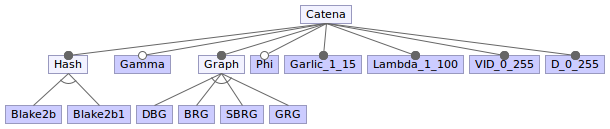
\includegraphics[width=0.8\textwidth]{images/Catena_Feature_model}
  \caption{Catena Feature Model.}
  \label{fm_catena}
\end{figure}

The Catena password hashing framework has eight features, three binary and 5 numerical (numerical features are represented by their name, min value and max value; separated with underscores). This results in a configuration space of \textbf{3,145,728,000} different possibilities (variants) to configure Catenas password hashing mode. We extracted the following features:

%Project size in Classes and Functions
%Project properties (SPL Model)
%Features explained
%Workload
%Num Dimensions: 3b 5n\todo{3+2b 4n}
%Whole configuration space: 3,145,728,000

\begin{description}[style=multiline,leftmargin=7em]
	\item [Hash] is a boolean parameter defining the used hash function.
	\item [Gamma] is a boolean parameter enabling the selection of a salt-dependent memory accesses layer to be resistant against attacks on dedicated hardware (e.g., ASICs\footnote{ASICs are hardware implementations of functions which are specialized to perform exactly a specific task.}).
	\item [Phi] is a boolean parameter enabling additional security properties\footnote{If Phi is enabled, Catena is resistant against parallel computations of hashes. But Phi has the drawback that Catena becomes vulnerable against other attacks \cite{10.1007/978-3-319-29938-9_7}.}.
	\item [Graph] defines one out of four different graph structures, which, in turn, defines the amount of necessary memory and time to compute the final hash.
	\item [Garlic] defines time and memory requirements in a range from 1 to 15.
	\item [Lambda] defines the depth of the graph in a range from 1 to one 100.
	\item [VID] decodes the unique version of Catena in a range from 0 to 255.
	\item [D] is an numerical parameter that is hashed together with other parameters to make up the tweak (increasing the additional computational effort for an adversary) in a range from 0 to two 255.
\end{description}

To execute Catena, we have to pick a configuration and we have to define a workload. A workload for Catena consists of three parameter: the password to be hashed, an user-defined salt, and the output length of the hash. Table~\ref{wl_catena} presents the three workloads we used. The first workload consists of an empty password string, an empty salt string, and an output length of one. With this workload we tried to minimize the amount of computations Catena has to perform. The second workload is exactly the half in each parameter and the last workload is an example workload we have taken from the Catena test vectors repository\footnote{The Catena test vactore are available on \url{https://github.com/medsec/catena-test-vectors}.}.

\begin{table}[h]
% Include Profiling Overhead and Accuracy to table

	\centering % Center table
    \begin{tabular}{*{9}{c}}
    	\toprule
        \# &Password & Salt & Output Length \\
        \midrule
        1 & '' & '' & 1 \\
        \midrule
        2 & '012345012345012345012345' & '6789ab6789ab' & 32 \\
        \midrule
        3 & \makecell{'012345012345012345012345'+ \\ '012345012345012345012345'} & \makecell{'6789ab6789ab'+ \\ '6789ab6789ab'} & 64 \\
        \bottomrule
    \end{tabular}
    \captionof{table}{Catena Workloads.}
    \label{wl_catena}
\end{table}


\subsection{H2}

% description
H2 is a database engine written in Java with the aim to be one of the fastest \ac{OSS} databases. In comparison to other databases (e.g., HSQLDB, Derby, PostgreSQL, and MySQL) H2 is faster but consumes more memory\footnote{Performance benchmark results and descriptions of the used test cases are available on \url{http://h2database.com/html/performance.html}.}.

% Configuration space extraction
The H2 project provides a detailed online documentation\footnote{Documentation of parameters is available on \url{http://h2database.com/javadoc/org/h2/engine/DbSettings.html}.} for configuration options, usage scenarios, benchmark results, and other useful information. We extracted the set of configuration options from the documentation and created the feature model (shown in Figure~\ref{fm_h2}). In total, we extracted fourteen binary options and two numerical options which result in a configuration space of 3,920,000,000 different variants. 

%Project description
%Project size in Classes and Functions
%Project properties (SPL Model)
%Features explained
%Workload
%Num dimensions: 14b 2n
%Whole configuration Space: 3,920,000,000

\begin{figure}[h]
  \centering
  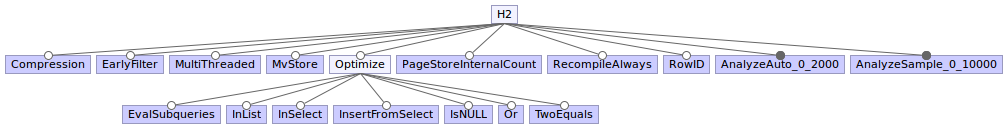
\includegraphics[width=\textwidth]{images/H2_Feature_model}
  \caption{H2 Feature Model.}
  \label{fm_h2}
\end{figure}

We excluded some options, because they does not influence the performance behaviour of the database (e.g., \textit{databaseToUpper} writes database names always in uppercase or \textit{defaultEscape} defines the default escape character) or produce exceptions during execution of the performance tests (e.g., changing the default value of \textit{maxQueryTimeout} causes some queries to not be executed). We extracted the following configuration options:

\begin{description}[style=multiline,leftmargin=11em]
	\item [Compression] compresses data when stored.
	\item [EarlyFilter] allows table implementations to apply filter conditions early on.
	\item [MultiThreaded] enables multi threading.
	\item [MvStore] enables the use of the MVStore storage engine.
	\item [OptimizeEvalSubqueries] optimizes subqueries that are independent of the outer query.
	\item [OptimizeInList] optimizes the \textit{IN(...)} and \textit{IN(SELECT ...)} operations.
	\item [OptimizeInSelect] optimizes the \textit{IN(SELECT ...)} operation.
	\item [OptimizeInsertFromSelect] enables insertion into tables from queries directly by passing temporary disc storage.
	\item [OptimizeIsNull] enables the use of indexing with \textit{IS NULL} checks.
	\item [OptimizeOr] optimizes the \textit{OR} operation.
	\item [OptimizeTwoEquals] enables the optimization of the equality check.
	\item [PageStoreInternalCount] enables updating the internal row counts.
	\item [RecompileAlways] enables that prepared statements always gets recompiled.
	\item [RowID] adds the pseudo-column \textit{\_ROWID\_} to each table.
	\item [AnalyzeAuto] is a number which defines the necessary number of changes of rows in a table before the table gets analyzed.
	\item [AnalyzeSample] is a number which defines how many samples of a table gets analyzed.
\end{description}

% workload is the size of the database [10,000; 55,000; 100,000]
% performance extraction functionality are the tests of the benchnmark
To create a meaningful workload, we vary the size of the data stored in the databased for each workload. To this end, we initialized the tables of the database with 10,000, 55,000, and 100,000 rows for the respective workloads. To generate load on the database, we use the benchmark that was provided by the vendor. This benchmark has been used previously to compare different database engines.

\subsection{Sunflow}

The third subject system is the rendering engine Sunflow. It is an \ac{OSS} written in Java. Sunflow is built around a ray tracing core to create photo-realistic images with the help of many different features such as camera motion blurring, lightmap generation, texture mapping, normal mapping, and other features. 

We analyze the performance of the process of rendering an image. Therefore, Sunflow already provides a benchmark which analyzes the resulting image (by time and by image quality) while modifying different parameters. We extracted all parameter that configure (\textit{DiffuseDepth},\textit{ReflectionDepth}, and \textit{RefractionDepth}) to create the feature model of Sonflow. Moreover, we identified three more parameters (\textit{Threads},\textit{BucketSize}, and \textit{Samples}) that were hard-coded in the source code of the benchmark. Although Sunflow provides additional configuration options for different use cases, we wanted to stick to the process of generating one image by using the standard scene (the cornell box with two tea pods and two glass balls).

\begin{figure}
  \centering
  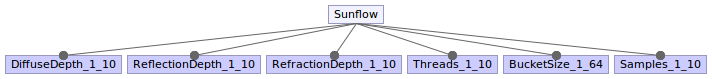
\includegraphics[width=\textwidth]{images/Sunflow_Feature_model}
  \caption{Sunflow Feature Model.}
  \label{fm_sunflow}
\end{figure}

In total, we have a configuration space of 6,400,000 variants. In the following, we present a short description of all configuration options we used:

%Project description
%Project size in Classes and Functions
%Project properties (SPL Model)
%Features explained
%Workload
%Num dimensions: 6n
%Whole configuration space: 6,400,000

\begin{description}[style=multiline,leftmargin=11em]
	\item [DiffuseDepth] controls the maximum depth of diffuse light paths in the scene. 
	\item [ReflectionDepth] controls the maximum number of reflections a ray can do in the scene.
	\item [RefractionDepth] controls the maximum number of refractions a ray can do in the scene.
	\item [Threads] number of threads used for calculating the image in parallel.
	\item [BucketSize] defines the size of a moving window.
	\item [Samples] specifies the number of times the scene gets rendered.
\end{description}

As the different levels of workload, we vary the resolution of the generated image (64x64 pixel, 128x128 pixel, and 256x256 pixel).


In total we performed 21.000 measurements with each subject system. That is made up of 1000 random sampled configurations, 3 different workloads, and 7 repetitions of the measurement. We parallelepiped the measurements of the three subject systems, but at the end, we measured a total of 21 days for each subject system in parallel. During this time, we collected 100 GB of profiling data. 


\section{Results}
\label{results}
% Present raw results and answer RQs

In the following we present the results of this thesis. %We show how much of the performance we were able to describe with our approach. %Subsequently, we analyze the the results with respect their significance.

%Catena wl 
%0: 50
%learned 413.0315849151743
%unlearn 412.2929499999999
%wl 1: 50
%learned 412.27993013030084
%unlearn 410.4239999999998
%wl 2: 50
%learned 414.49257749353643
%unlearn 412.6332999999999

%H2 wl 
%0: 50
%learned 29525.66128965314
%unlearn 29508.411648498375
%wl 1: 50
%learned 128143.5496972018
%unlearn 128117.78896533113
%wl 2: 50
%learned 86365.01659749153
%unlearn 86335.04998479395

%Sunflow 
%wl 0: 51
%learned 551.0664122092193
%unlearn 534.0370174946153
%wl 1: 51
%learned 552.7638023036519
%unlearn 523.5586365656109
%wl 2: 51
%learned 517.6968025194329
%unlearn 494.82592202380863


\subsection{Performance-influence Models at Method Level}
\label{perf_infl_models_m_lvl}

To learn the influence of the individual configuration options on performance, we applied the regression models presented in section~\ref{lin_reg}. Before we start training the model, we check if we have enough data to train and test the model. We learn out models only for methods if we have at least 11 measurements. 

\begin{table}[h]
	\centering % Center table
    \begin{tabular}{*{9}{l}}

        Input (Features + Interactions) & Output (Performance) \\
        \toprule

        < $f_1, f_2, f_3, f_4, f_5, f_6, f_7, f_8, f_{1,2}, f_{1,3}, ...$> & perforamcne \\
       
        < 0, 0, 1, 0, 10, 36, 144, 48, 0, 0, ... > & 345.75 \\
		< 0, 0, 1, 0, 11, 1, 144, 35, 0, 0, ... > & 30.1 \\
		< 0, 0, 1, 0, 12, 25, 213, 200, 0, 0, ... > & 1129.5 \\
		... & ...\\

    \end{tabular}
    \captionof{table}{Catena -- Example Input/Output Vector.}
    \label{table:example:inp_outp}
\end{table}

An example set of input--output vectors is shown in Figure~\ref{table:example:inp_outp}. To build the input vector for our regression models, we encoded the configuration as input, extended this input vector by all pair-wise interactions of the configuration options, and learned the corresponding performance value of the method.


\begin{table}[h]
	\centering % Center table
    \begin{tabular}{c c c c}

         		& Workload 1 & Workload 2 & Workload 3 \\

        Catena 	& 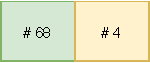
\includegraphics[width=.15\linewidth]{images/resCatenaWL1} & 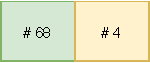
\includegraphics[width=.15\linewidth]{images/resCatenaWL1} & 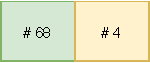
\includegraphics[width=.15\linewidth]{images/resCatenaWL1} \\

        H2 		& 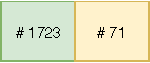
\includegraphics[width=.15\linewidth]{images/resH2} & 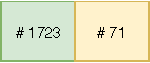
\includegraphics[width=.15\linewidth]{images/resH2} & 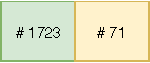
\includegraphics[width=.15\linewidth]{images/resH2} \\

        Sunflow & 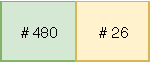
\includegraphics[width=.15\linewidth]{images/resSunflow} & 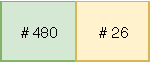
\includegraphics[width=.15\linewidth]{images/resSunflow} & 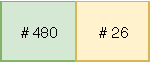
\includegraphics[width=.15\linewidth]{images/resSunflow} \\

    \end{tabular}
    \captionof{table}{Proportion of Learned Performance of \# Methods.}
    \label{table:res:learning}
\end{table}

We trained each method with all regression techniques and assessed their individual prediction accuracy by predicting all configurations in our test set. The result of the training process is shown in Table~\ref{table:res:learning}. This table visualizes the proportion of performance that we have learned (green) with our model, in contrast to the performance that we could not learn (yellow). Each field consists of the number of methods (\#) that together make up the portion of performance. It is noticeable, that we are able to predict half of the performance of each system with each workload even if we can assess the performance of about 95\% of the methods. 

\begin{figure}[h]
	\centering
	\begin{subfigure}{.49\textwidth}
	  \centering
	  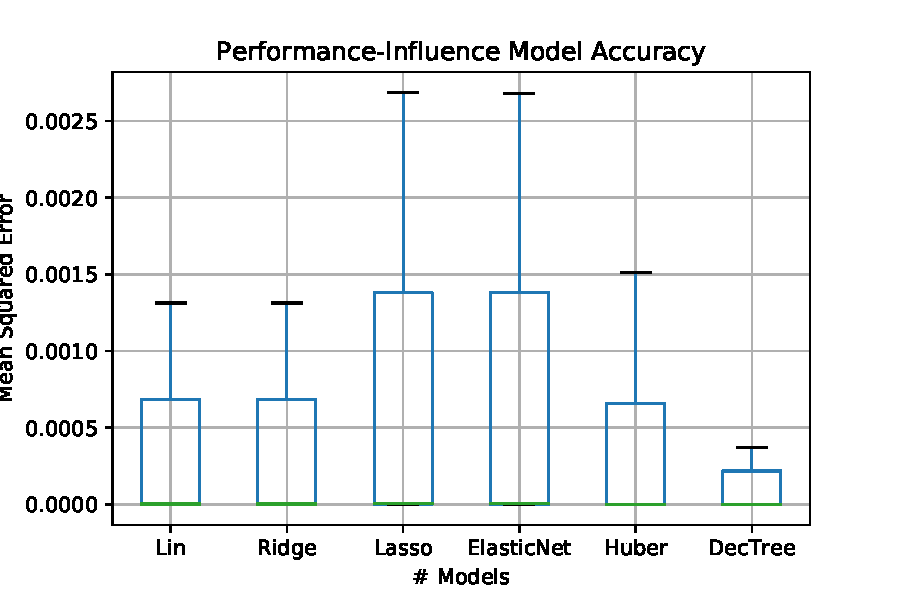
\includegraphics[width=\textwidth]{images/Catena_box_regression_model_overview_without_outl}
	  %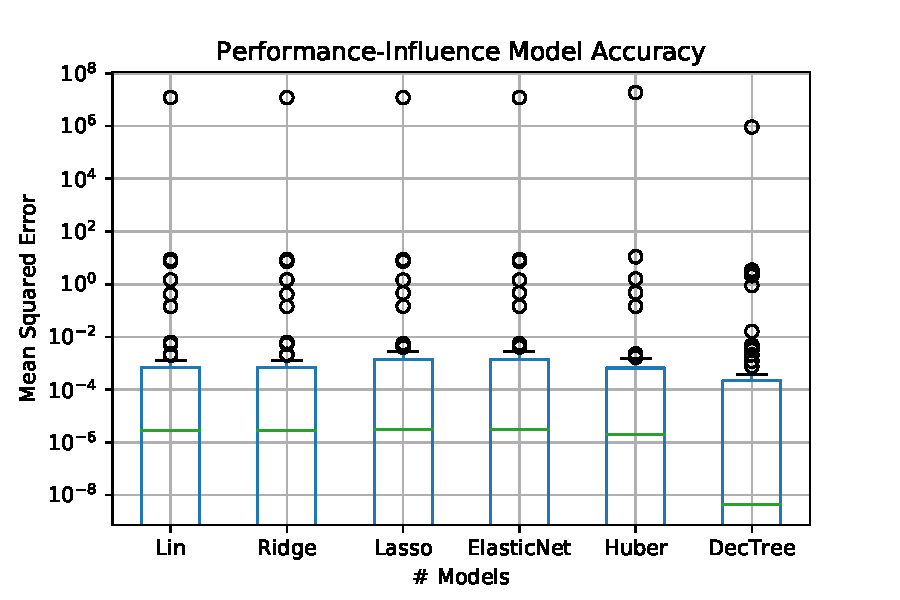
\includegraphics[width=0.7\textwidth]{images/Catena_box_regression_model_overview_with_outl_log}
	  \caption{Catena -- Prediction Error.}
	  \label{box_model_cross_comp_catena}
	\end{subfigure}
	\begin{subfigure}{.49\textwidth}
	  \centering
	  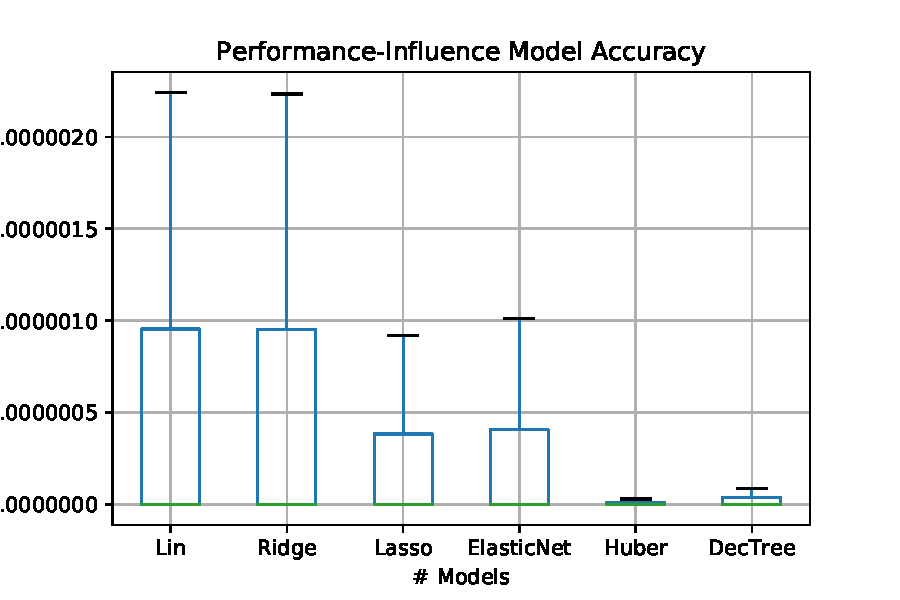
\includegraphics[width=\textwidth]{images/H2_box_regression_model_overview_without_outl}
	  %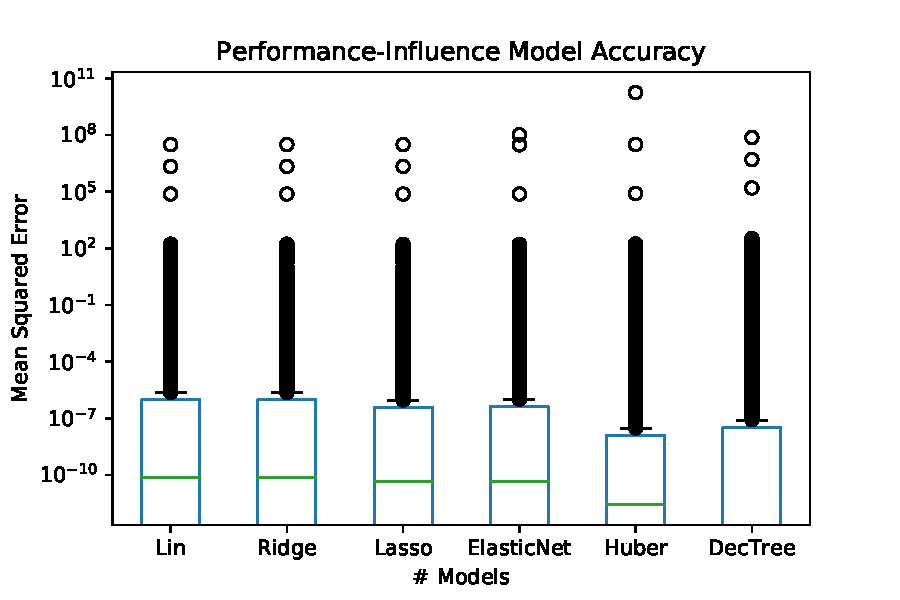
\includegraphics[width=0.7\textwidth]{images/H2_box_regression_model_overview_with_outl}
	  \caption{H2 -- Prediction Error.}
	  \label{box_model_cross_comp_h2}
	\end{subfigure}
	\begin{subfigure}{.49\textwidth}
	  \centering
	  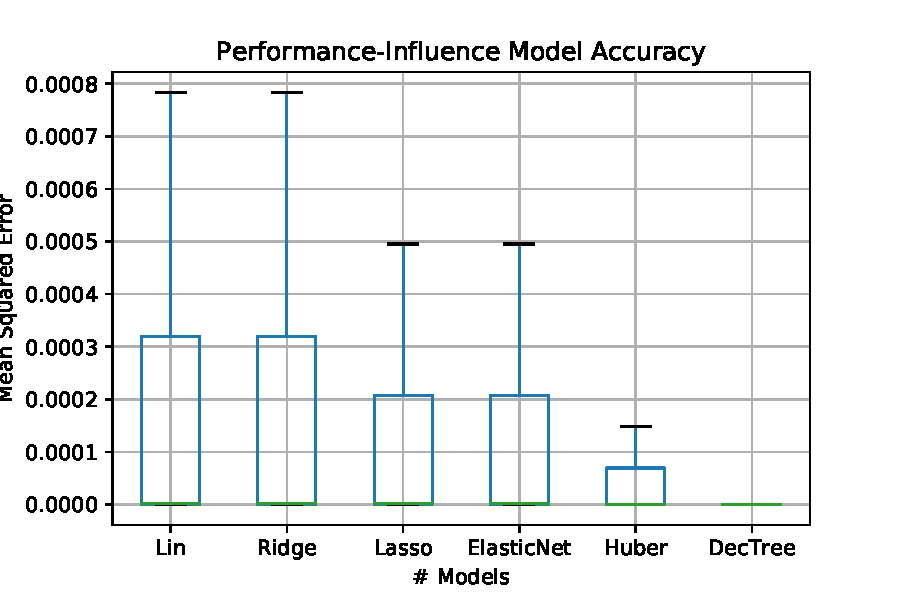
\includegraphics[width=\textwidth]{images/Sunflow_box_regression_model_overview_without_outl}
	  %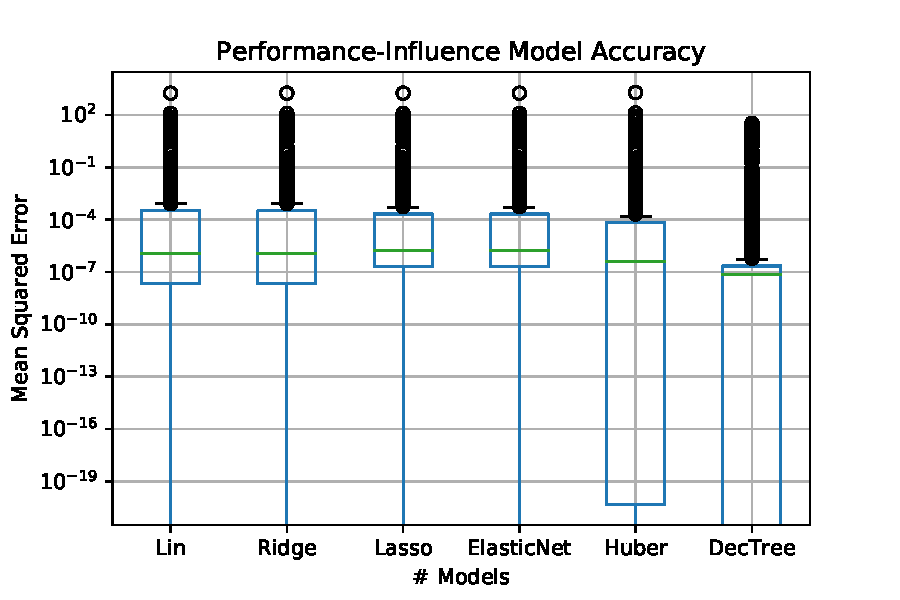
\includegraphics[width=0.7\textwidth]{images/Sunflow_box_regression_model_overview_with_outl_log}
	  \caption{Sunflow -- Prediction Error.}
	  \label{box_model_cross_comp_sunflow}
	\end{subfigure}
	\caption{Comparison of Prediction Error over all Subject Systems and Regression Model without Outliers.}
	\label{fig:regression_model_error_comparison}
\end{figure}

An overview of the regression models is presented in Figure~\ref{fig:regression_model_error_comparison}. Here, each boxplot comprises the error of all methods that we tried to learn with the individual regression models. We can see, that the median error of all models over all subject systems is close to zero. We also see that Linear Regression and Ridge Regression as well as Lasso and Elasic Net perform almost equally. But Huber Regression is always better than former regression models. With decision trees, we achieve the best results of prediction performance by configuration. But it is not possible to get the influence of the individual features or interactions with decision trees.


Next, we analyze the errors of the regression techniques that predict the performance of a method. Therefore, we assessed the \acp{MSE} between the predicted and the actual performance values of each method using the test set. We utilized the technique with the smallest error, to have always the best for further evaluation. To provide a better illustrate the error distribution, we split the figures by 10\% prediction error.

\begin{figure}[h]
	\centering
	\begin{subfigure}{.5\textwidth}
	  \centering
	  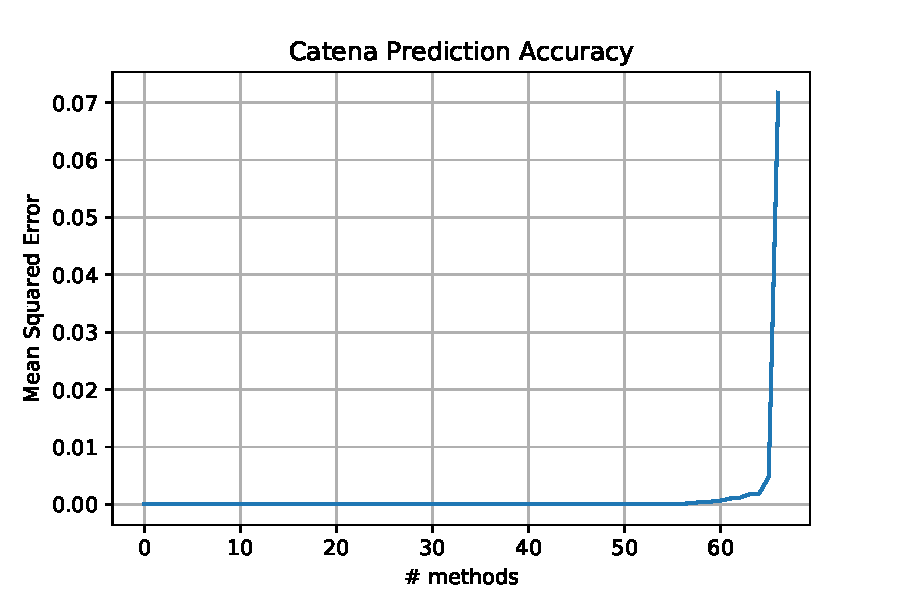
\includegraphics[width=.99\linewidth]{images/Catena_plt_learnable_func_all_model_mse}
	  \caption{Learned Methods.}
	  \label{fig:catena_model_mse_lern}
	\end{subfigure}%
	\begin{subfigure}{.5\textwidth}
	  \centering
	  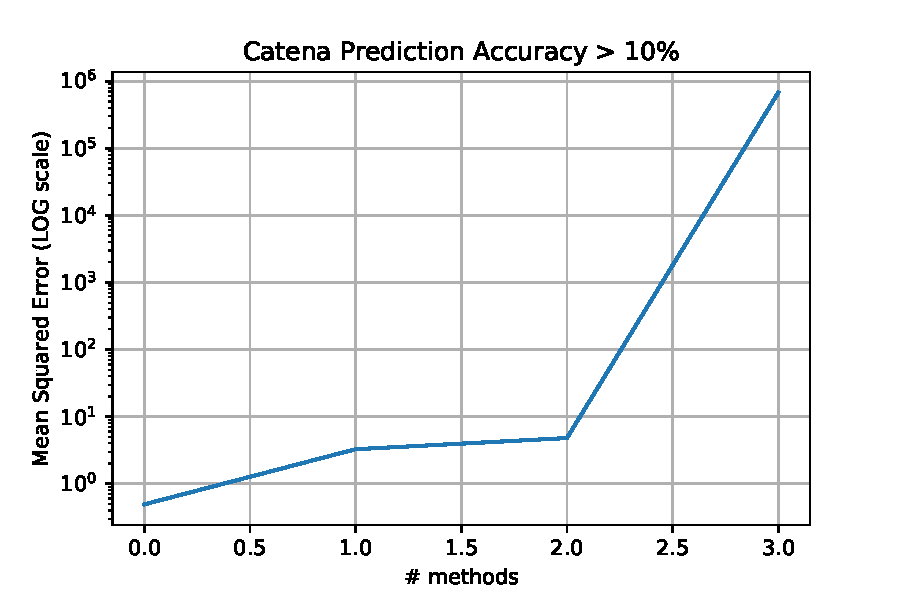
\includegraphics[width=.99\linewidth]{images/Catena_plt_unlearnable_func_all_model_mse_log}
	  \caption{Unlearned Methods.}
	  \label{fig:catena_model_mse_unlern}
	\end{subfigure}
	\caption{Catena -- Comparison of Learnability over all methods (\#72).}
	\label{fig:c_lernability_all_methods}
\end{figure}

For Catena we had in total 82 methods available for learning. We had to exclude 10 of them from our learning approach, because they got less than 11 times executed under different configurations. The results of learning the influence of the remaining 72 methods are shown in Figure~\ref{fig:c_lernability_all_methods}. In Figure~\ref{fig:catena_model_mse_lern}, we show the 68 methods that we are able to learn with an \ac{MSE} of less than 10\%. Also the 23 methods which are not influenced by any configuration option (presented in Section~\ref{conf_sens} and in Appendix~\ref{app:conf:sens:catena}) belong to those methods. Nevertheless, we were not able to predict the performance of 4 methods, that makes 5.5\% out of all methods available for learning. These methods are presented in Figure~\ref{fig:catena_model_mse_unlern} aligned with an logarithmic \ac{MSE}. Later (in Section~\ref{discussion}), we discuss possible reasons why we could not learn these methods.
%Catena 10 methods with too less data -> 72
%67 learnable
%5 not learned 6.9% of all

\begin{figure}[h]
	\centering
	\begin{subfigure}{.5\textwidth}
	  \centering
	  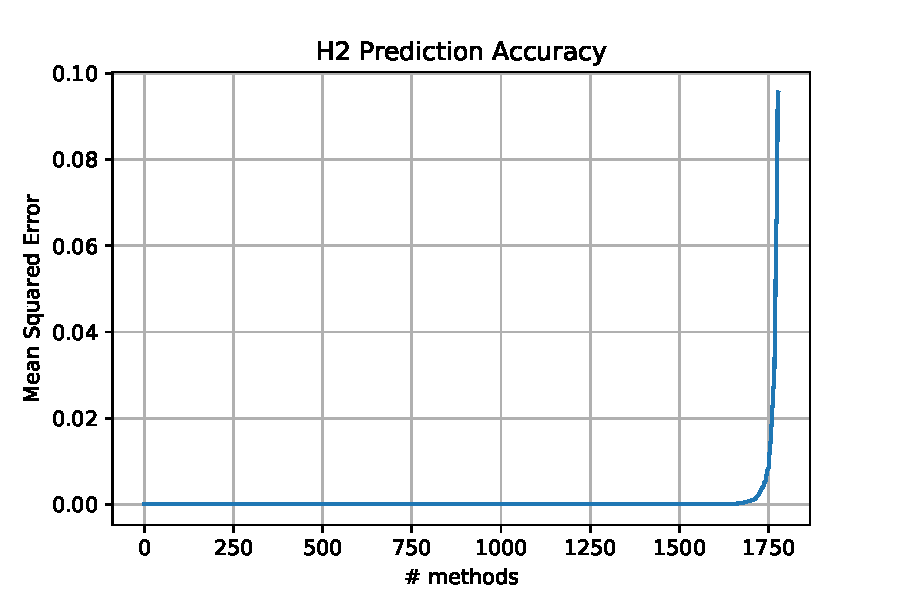
\includegraphics[width=.99\linewidth]{images/H2_plt_learnable_func_all_model_mse}
	  \caption{Learned Methods.}
	  \label{fig:h2_model_mse_lern}
	\end{subfigure}%
	\begin{subfigure}{.5\textwidth}
	  \centering
	  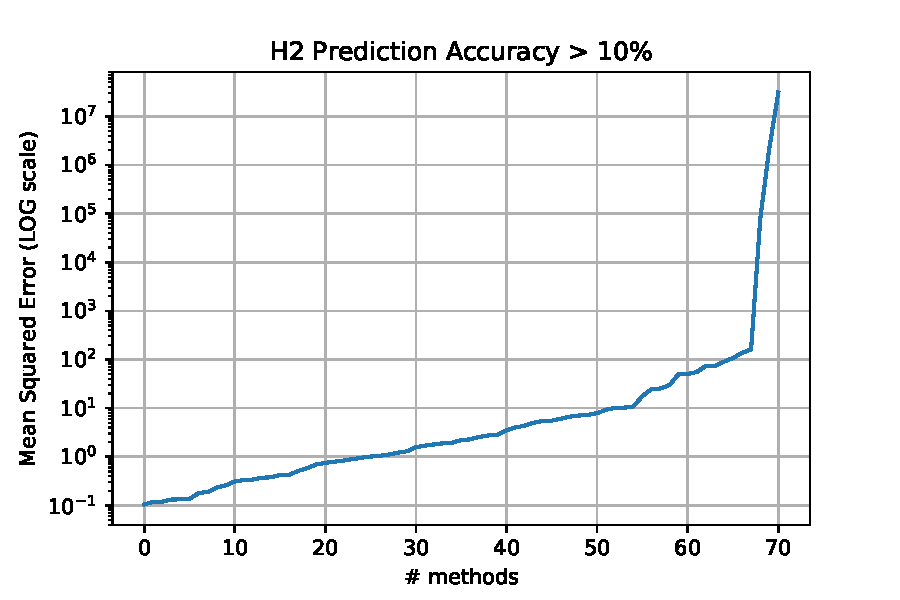
\includegraphics[width=.99\linewidth]{images/H2_plt_unlearnable_func_all_model_mse_log}
	  \caption{Unlearned Methods.}
	  \label{fig:h2_model_mse_unlern}
	\end{subfigure}
	\caption{H2 -- Comparison of Learnability over all methods (1850\#).}
	\label{fig:h_lernability_all_methods}
\end{figure}

Figure~\ref{fig:h_lernability_all_methods} shows the results of the learning the influence of configuration options of H2. In total, we had 1865 methods available from which we excluded 15 methods because of the lack of data. We were able to predict the performance of 1794 methods, but just like with Catena, we are not able to predict 3.8\% (71) of the methods with an \ac{MSE} of less than 10\%. Figure~\ref{fig:h2_model_mse_unlern} also show that the error of 5 methods increases very strong. 

%H2:
%- 1865 methods in total
%- 15 methods with too less data
%- 71 methods unlearned 3,8\%

\begin{figure}[h]
	\centering
	\begin{subfigure}{.5\textwidth}
	  \centering
	  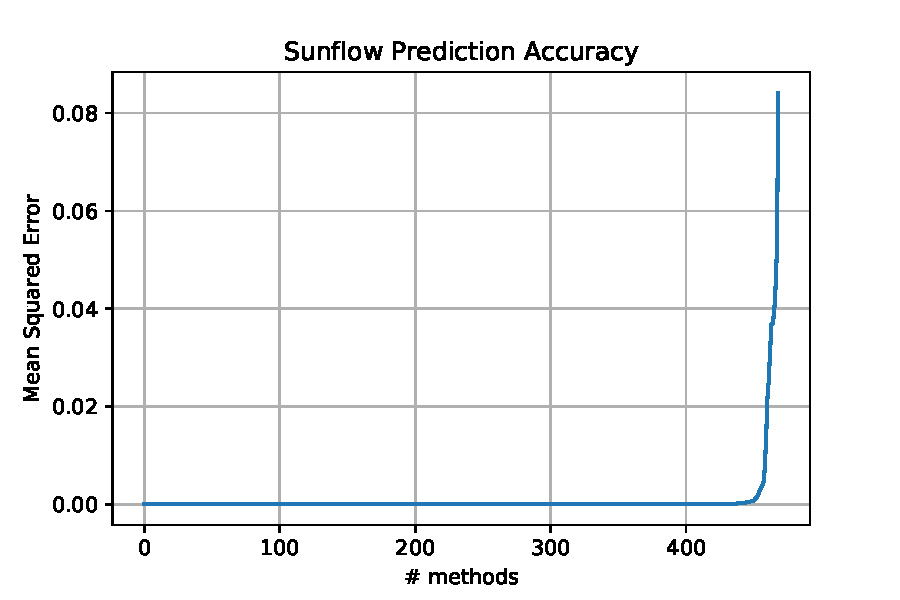
\includegraphics[width=.99\linewidth]{images/Sunflow_plt_learnable_func_all_model_mse}
	  \caption{Learned Methods.}
	  \label{fig:sunflow_model_mse_lern}
	\end{subfigure}%
	\begin{subfigure}{.5\textwidth}
	  \centering
	  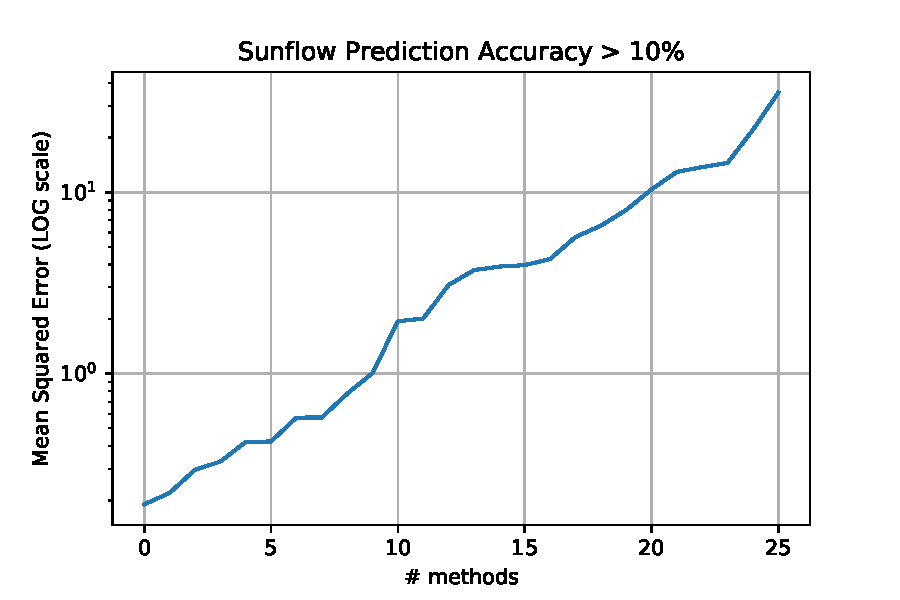
\includegraphics[width=.99\linewidth]{images/Sunflow_plt_unlearnable_func_all_model_mse_log}
	  \caption{Unlearned Methods.}
	  \label{fig:sunflow_model_mse_unlern}
	\end{subfigure}
	\caption{Sunflow -- Comparison of Learnability over all methods (\#496).}
	\label{fig:s_lernability_all_methods}
\end{figure}

The results of learning the influence of Sunflow are shown in Figure~\ref{fig:s_lernability_all_methods}. We tried to learn 496 methods (we had to exclude 10 methods) from which we are able to predict 480. Again, we were not able to predict the performance of 26 methods (which are 5.1\%). But in contract to the unlearned methods of Catena and H2, the \ac{MSE} increases nearly linear.

%Sunflow:
%- 506 methods in total
%- 10 methods with too less data
%- 26 methods unlearned 5.1\%

\begin{figure}[h]
	\centering
	\begin{subfigure}{.5\textwidth}
	  \centering
	  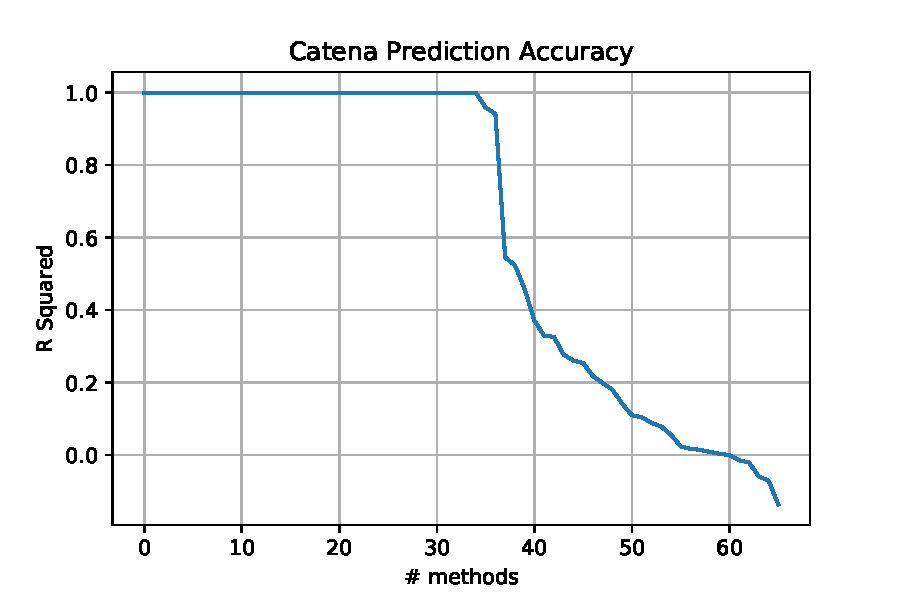
\includegraphics[width=.99\linewidth]{images/Catena_plt_learnable_func_all_model_r_sq}
	  \caption{Catena -- R squared.}
	  \label{fig:catena_model_r_sq}
	\end{subfigure}%
	\begin{subfigure}{.5\textwidth}
	  \centering
	  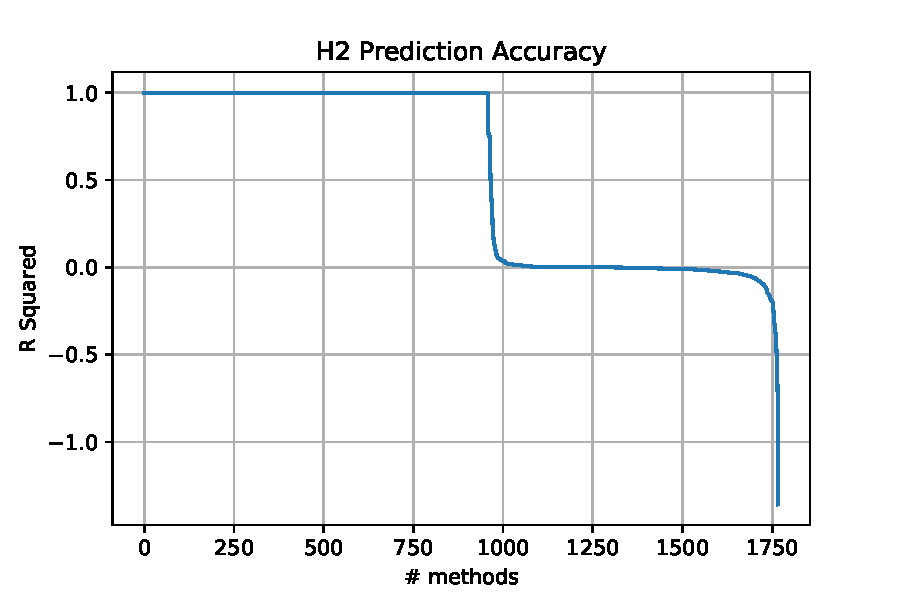
\includegraphics[width=.99\linewidth]{images/H2_plt_learnable_func_all_model_r_sq}
	  \caption{H2 -- R squared.}
	  \label{fig:catena_model_r_sq}
	\end{subfigure}
	\begin{subfigure}{.5\textwidth}
	  \centering
	  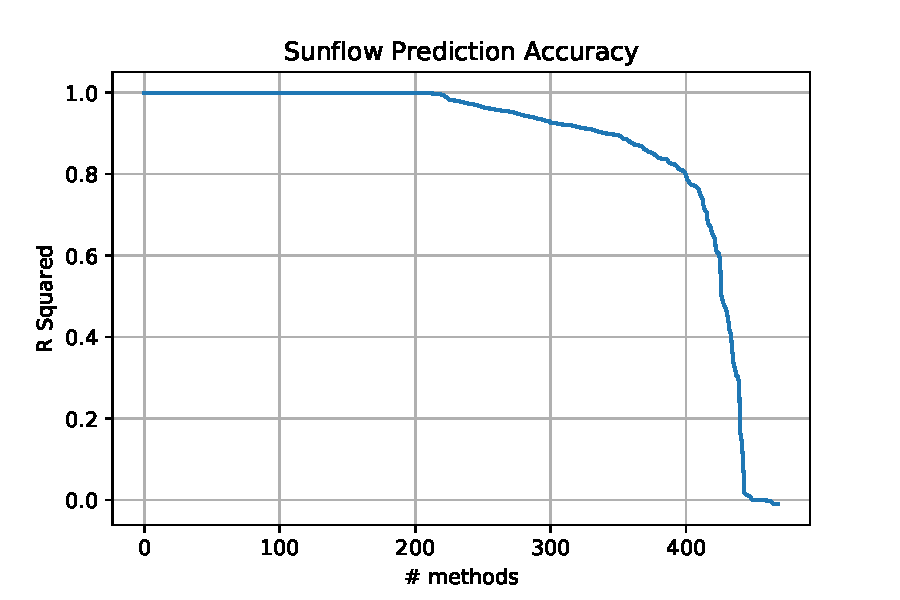
\includegraphics[width=.99\linewidth]{images/Sunflow_plt_learnable_func_all_model_r_sq}
	  \caption{Sunflow -- R squared.}
	  \label{fig:catena_model_r_sq}
	\end{subfigure}
	\caption{Performance-Influence Model Validation.}
	\label{fig:c_lernability_all_methods}
\end{figure}

To evaluate how much of the variance in the data we can explain with out models, we assessed the R squared coefficient of each model for the methods of the subject systems. Figure~\ref{fig:c_lernability_all_methods} shows proportion of the variance in the performance values that is predictable from the configurations. We can see, that the R squared score of the methods of each subject system goes beyond zero. This indicates that, especially with the methods whose score is beyond zero, all regression techniques of our model are not able to explain the performance based on the configuration. Hence, we are not able to predict the performance values of the affected methods. That coincides with our observations of the sum of squared errors (also called: sum of squared residuals) in Figures~\ref{fig:s_lernability_all_methods}, \ref{fig:h_lernability_all_methods}, and \ref{fig:c_lernability_all_methods}.



\subsection{Configuration Sensitivity}
\label{conf_sens}

To assess the sensitivity of each individual method regarding the chosen configuration of the respective configurable software system, we calculated the difference in the performance values of the methods over each configuration. To this end, we calculated the standard deviation of the performance values to get the amount of variation of the performance of each method depending on the configurations. Then, we divided the standard deviation by the mean to calculate the \ac{CV}\footnote{\ac{CV} is also known as the relative standard deviation, which describes the ration of standard deviation to the mean. Values above 1 does have a high variance, which describes in our case a high configuration sensitivity}.

\begin{figure}[h]
	\centering
	\begin{subfigure}{.5\textwidth}
	  \centering
	  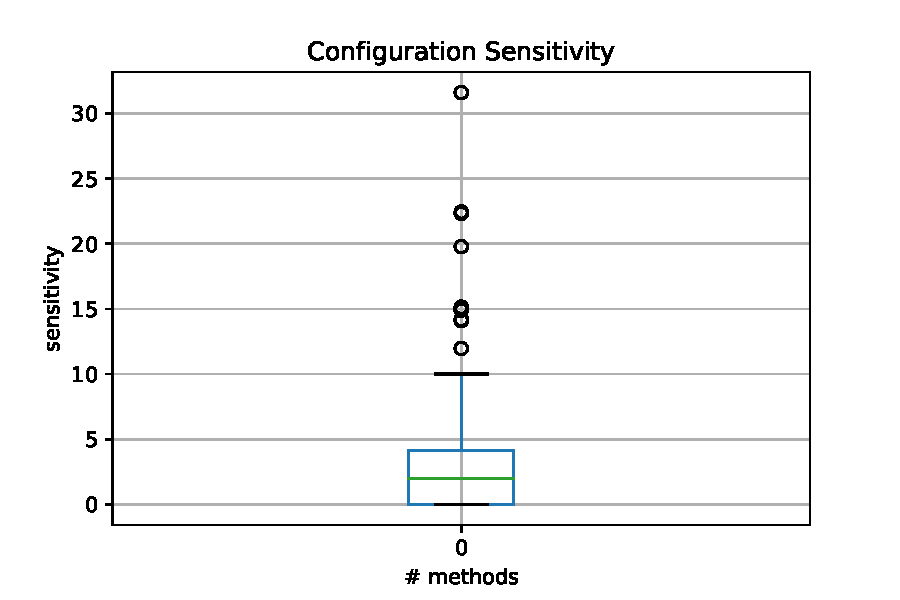
\includegraphics[width=.99\linewidth]{images/Catena_box_conf_sens_cv_with_outl}
	  \caption{Boxplot with Outliers.}
	  \label{fig:c_conf_sens_on_method:sub1}
	\end{subfigure}%
	\begin{subfigure}{.5\textwidth}
	  \centering
	  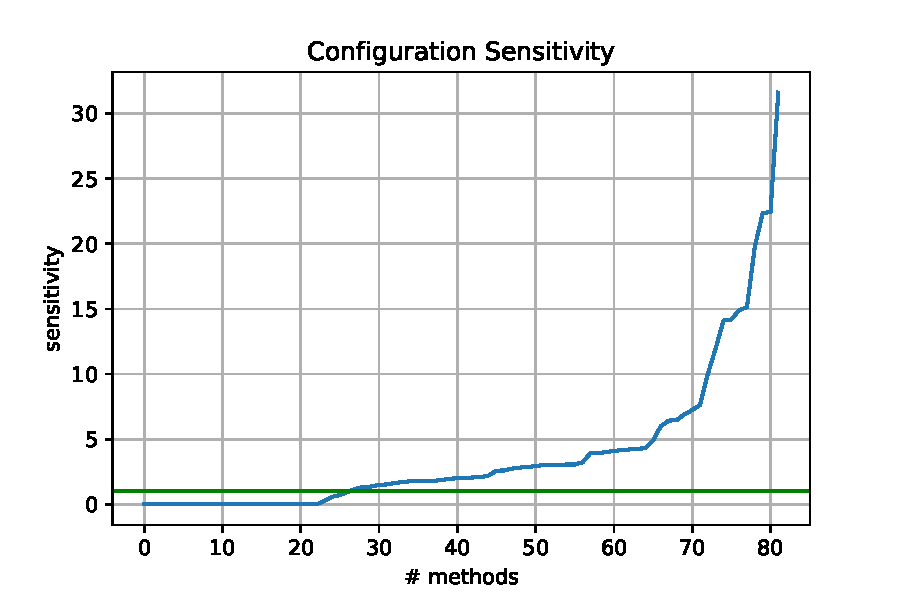
\includegraphics[width=.99\linewidth]{images/catena_plt_conf_sens_cv_with_outl}
	  \caption{Whole Distribution}
	  \label{fig:c_conf_sens_on_method:sub2}
	\end{subfigure}
	\caption{Catena - Coefficient of Variation in Configuration Sensitivity of Methods (\#82).}
	\label{fig:c_conf_sens_on_method}
\end{figure}


Distribution of the relative standard deviations for each configuration of a specific workload.

We summarize the configuration sensitivity of the methods of Catena in Figure~\ref{fig:c_conf_sens_on_method}. The Subfigure~\ref{fig:c_conf_sens_on_method:sub1} shows the distribution of the \ac{CV}-values of all methods as a box plot with outliers. Subfigure~\ref{fig:c_conf_sens_on_method:sub2} marks the \ac{CV}-value of 1 (the green line). This value divides all methods into a configuration insensitive (below) area and configuration sensitive (above) area. We can see that there is a great difference in the configuration sensitivity of the different methods. Most methods are weak sensitive, but there are some methods which are heavily sensitive to different configuration options. That is, we observe that more than half of the methods' performance changes depending on the chosen configuration. 

\begin{figure}[h]
	\centering
	\begin{subfigure}{.5\textwidth}
	  \centering
	  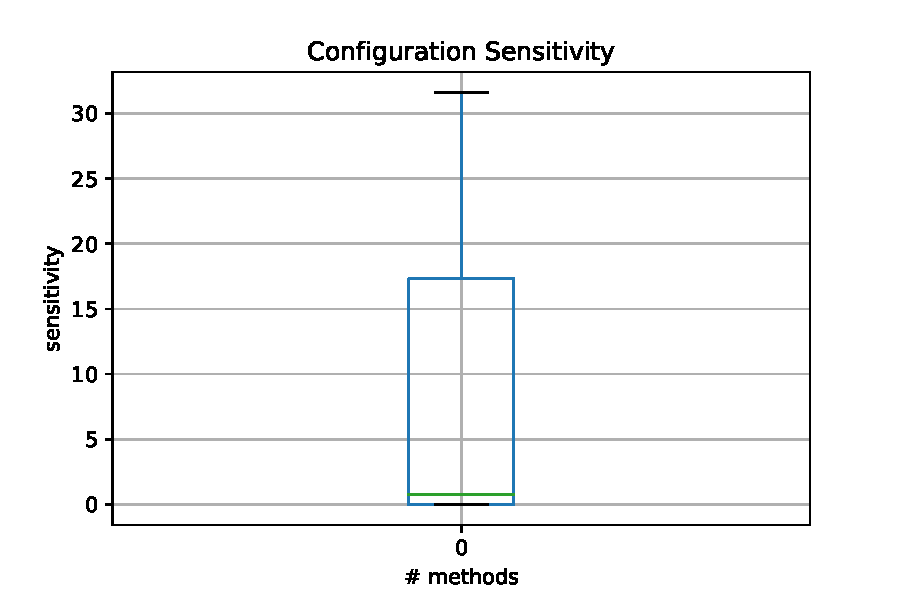
\includegraphics[width=.99\linewidth]{images/H2_box_conf_sens_cv_with_outl}
	  \caption{Boxplot with Outliers.}
	  \label{fig:h_conf_sens_on_method:sub1}
	\end{subfigure}%
	\begin{subfigure}{.5\textwidth}
	  \centering
	  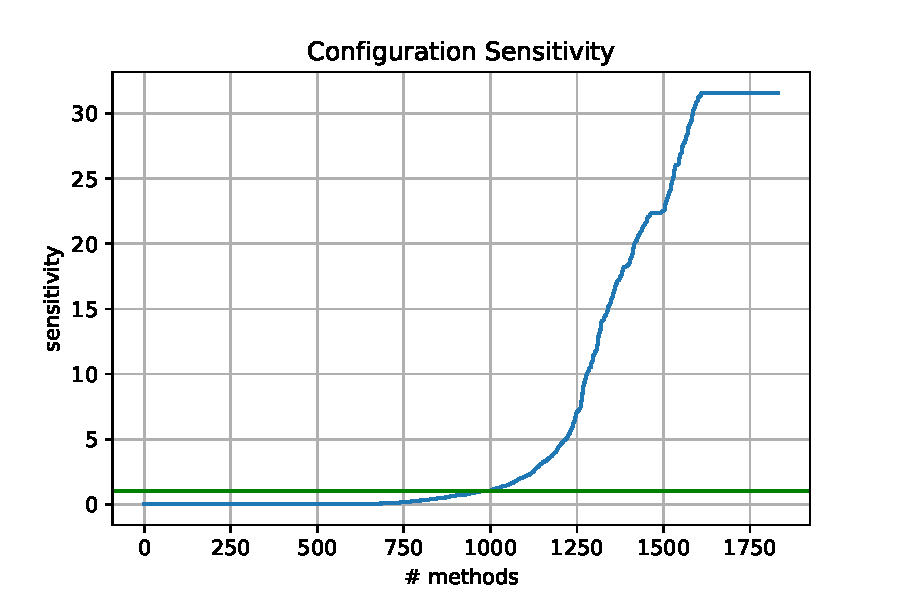
\includegraphics[width=.99\linewidth]{images/H2_plt_conf_sens_cv_with_outl}
	  \caption{Whole Distribution}
	  \label{fig:h_conf_sens_on_method:sub2}
	\end{subfigure}
	\caption{H2 -- Coefficient of Variation in Configuration Sensitivity of Methods (\#1865).}
	\label{fig:h_conf_sens_on_method}
\end{figure}

The Figures~\ref{fig:h_conf_sens_on_method:sub1} and~\ref{fig:h_conf_sens_on_method:sub2} show the configuration sensitivity of the H2 database engine. We investigated the 1850 methods that are executed during the test cases. We observe, that about half of the methods are weak sensitive to different configurations, which is shown by the height of the mean in the box plot and the \ac{CV}-marker line. For the remaining methods, the sensitivity increases rapidly until they plateau, where around 250 methods does have the same sensitivity. 

\begin{figure}[h]
	\centering
	\begin{subfigure}{.5\textwidth}
	  \centering
	  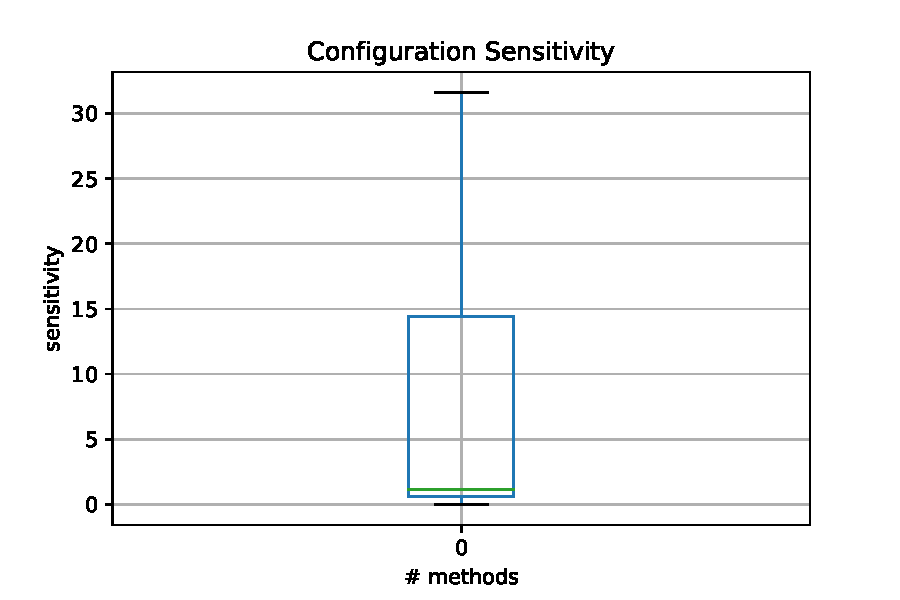
\includegraphics[width=.99\linewidth]{images/Sunflow_box_conf_sens_cv_with_outl}
	  \caption{Boxplot with Outliers.}
	  \label{fig:s_conf_sens_on_method:sub1}
	\end{subfigure}%
	\begin{subfigure}{.5\textwidth}
	  \centering
	  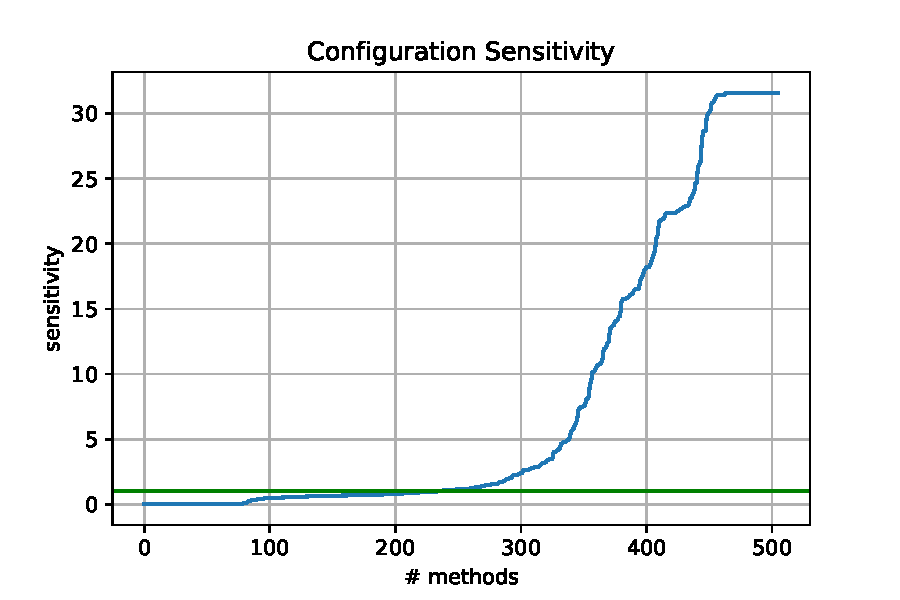
\includegraphics[width=.99\linewidth]{images/Sunflow_plt_conf_sens_cv_with_outl}
	  \caption{Whole Distribution}
	  \label{fig:s_conf_sens_on_method:sub2}
	\end{subfigure}
	\caption{Sunflow -- Coefficient of Variation in Configuration Sensitivity of Methods (\#506).}
	\label{fig:s_conf_sens_on_method}
\end{figure}

The configuration sensitivity of the methods of the rendering engine Sunflow is shown in the Figures~\ref{fig:s_conf_sens_on_method:sub1} and~\ref{fig:s_conf_sens_on_method:sub2}. Again, half of the methods are insensitive to the chosen configuration. Furthermore, the sensitivity increases rapidly until a plateau with the highest sensitivity. The difference to H2 is that there are less methods with no sensitivity, but more methods that are weak sensitive.



\subsection{External Measurement Influence}
\label{ext_measurement_infl}

External influences such as the garbage collector or operating-system processes can substantially influence the reliability of our fine-grained performance measurements. Remember that we measure at method level with a resolution within milliseconds. For example, a context switch in the operating system can lead to severe measurement bias. Hence, we restricted possible sources of non-determinism to reduce their influence (fixed the hardware setup and minimal amount of installed software. To further quantify the remaining influence of measurement bias, we repeated each test case 7 times.

\begin{figure}[h]
  \centering
  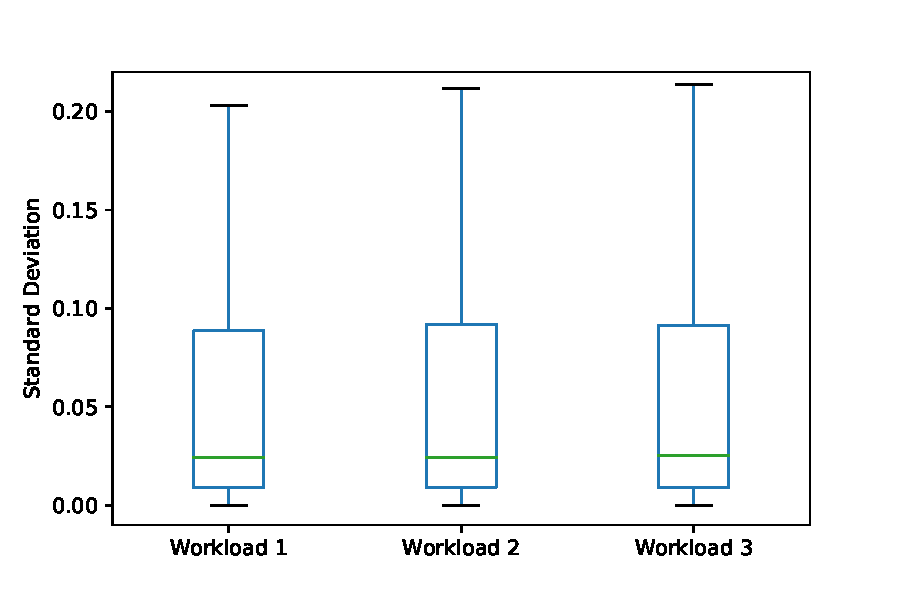
\includegraphics[width=0.6\textwidth]{images/catena_m_infl_wl_012}
  \caption{Catena - Distribution of the relative standard deviations for each configuration of a specific workload.}
  \label{box_measure_infl_catena}
\end{figure}

Figure~\ref{box_measure_infl_catena} shows the standard deviation of Catena for the three defined workloads (defined in Section~\ref{wl_catena}) for all sampled configurations using box plots. In about half of the configurations the mean relative standard deviation is only about 2.4\%. Furthermore, changing the workload does not influence the measurement bias.

\begin{figure}[h]
  \centering
  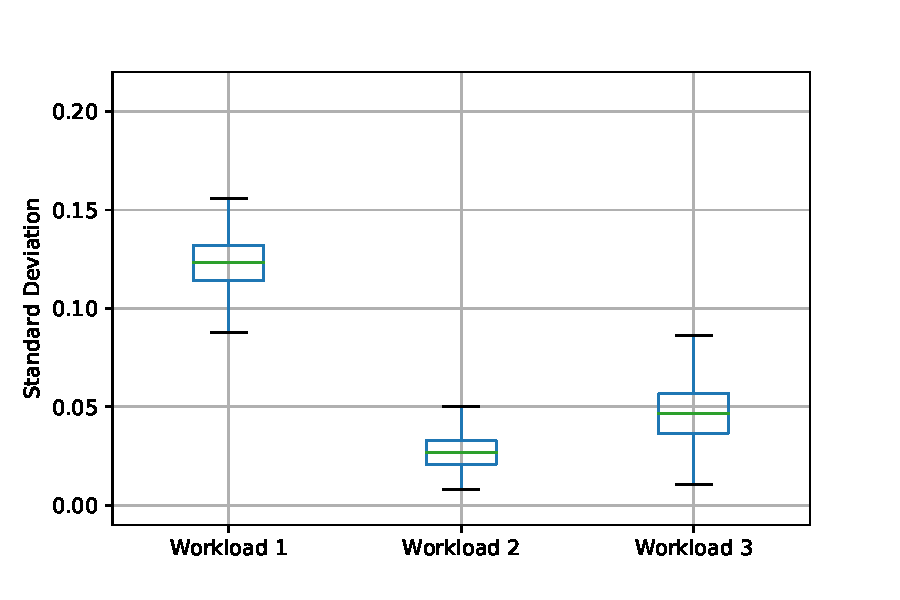
\includegraphics[width=0.6\textwidth]{images/h2_m_infl_wl_012}
  \caption{H2 - Distribution of the relative standard deviations for each configuration of a specific workload.}
  \label{box_measure_infl_h2}
\end{figure}

For H2, the picture changes. Figure~\ref{box_measure_infl_h2} shows that there is a difference in the variance of the standard deviations depending on the used workload. The variance of the standard deviations is the biggest with the fist workload, the lowest with the second workload. We believe that with increasing runtime the relative influence of measurement bias decreases. For example, JIT compilation should have the highest influence at the start of the program and the longer the program runs, the smaller is the relative influence on the overall runtime.

\begin{figure}[h]
  \centering
  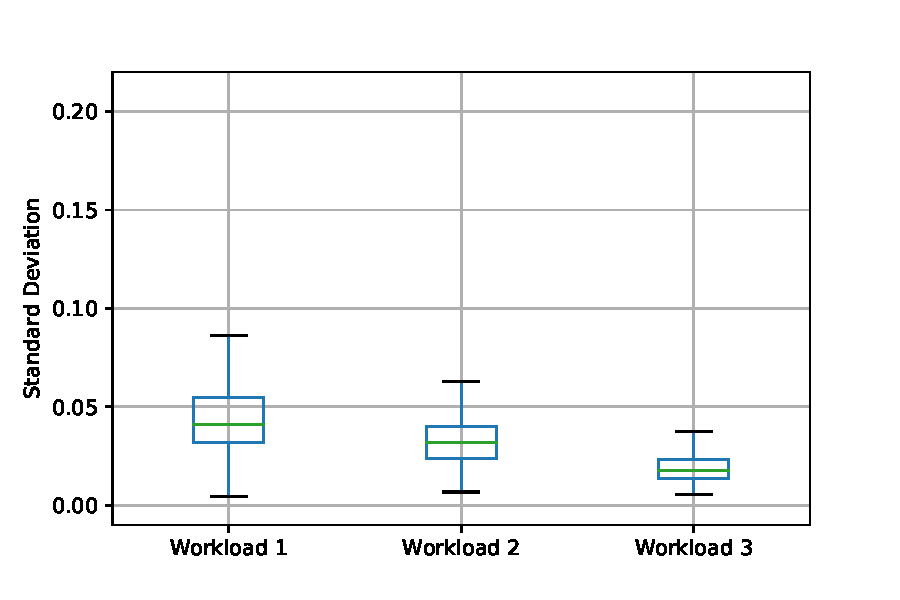
\includegraphics[width=0.6\textwidth]{images/sunflow_m_infl_wl_012}
  \caption{Sunflow - Distribution of the relative standard deviations for each configuration of a specific workload.}
  \label{box_measure_infl_sunflow}
\end{figure}

For Sunflow, we see a similar picture as for H2 (cf.~\ref{box_measure_infl_sunflow}). The influence of external factors, as well as the variance in the influences decrease from the first workload to the third.

\begin{figure}[h]
  \centering
  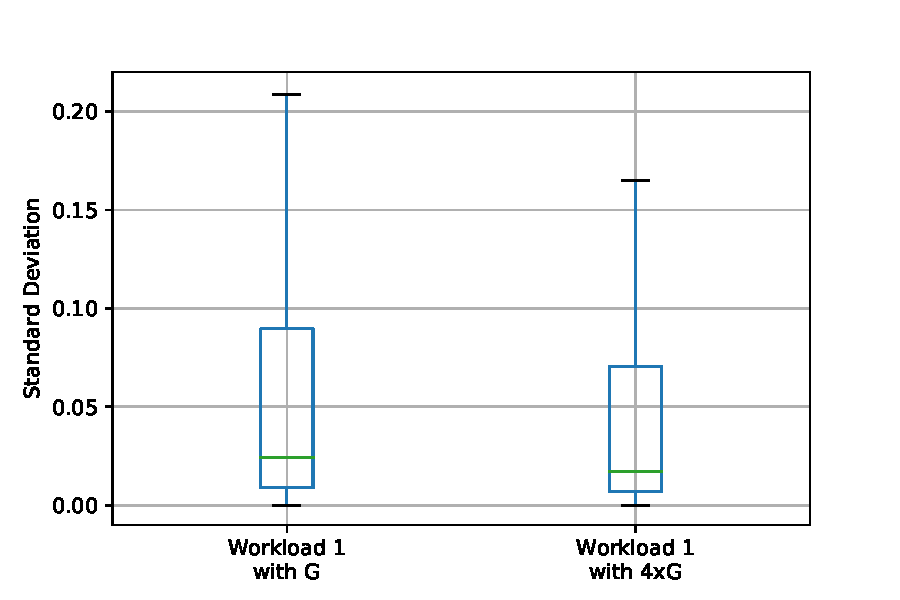
\includegraphics[width=0.6\textwidth]{images/catena_m_infl_wl_and_wlx4_0}
  \caption{Catena - Measurement Influence with all Configurations (\#820).}
  \label{box_measure_infl_catena_x4}
\end{figure}

Since Catenas measurement variance remains the same for all workloads, we changed the parameter \textit{Garlic} from a maximum of 15 to 17 (only for this experiment). Hereafter, the tests run for four times the time (increasing \textit{Garlic} by one doubles the runtime). We observed now a similar trend as for the other subject systems: a decrease in the measurement bias.

Analyzing the measurement bias shows that there is a proportion of non-determinism in our measurements over all subject systems and workloads. Overall, we can see that for all subject systems the measurement bias is low (usually between 2\% and 6\%) such that we conclude that we obtain robust and reproducible performance measurements.



\clearpage

\section{Discussion}
\label{discussion}


\rqparagraph{\ref{rq:perf_infl_model} \textit{How accurate are performance-influence models at method level learned by different techniques?}}

% fraction of learned performance? what have we learned?
In order to answer \ref{rq:perf_infl_model} we learned the influence of configuration options of three software systems for each of their methods. Therefore, we created a dataset, which combines each configuration option and each pair-wise combination of these options as independent variables and the performance of each method as dependent variable. We utilize different regression techniques to model the performance of each method. By picking the best regression technique per method, we are able to learn the performance of about 95\% of the methods. For about 5\% of the methods (Catena: 5.5\%, H2: 3.8\%, and Sunflow: 5.1\%), our model was not able to predict within an acceptable precision. 
But it is noticeable that, while successfully learning the performance-influence models of 95\% of the methods, we are only able to explain half of the performance of each system. To this end, we identified the performance hot-spots of the three subject systems: These 5\% of methods that we could not learn with our model are also those, which together unite half of the performance. 


% reconciliation - überleitung
\rqparagraph{\ref{rq:learning influence} \textit{What influences the learning of performance-influence models?}}

For each subject system, we were not able to learn the performance of about 5\% of the methods. \ref{rq:learning influence} will explain possible sources that influence the learning process. Therefore, we investigate the methods of Catena (overview in Table~\ref{tbl:unlearnable_methods_catena}) which we are unable to learn. 

Table~\ref{tbl:unlearnable_methods_catena} presents the five methods which are above our error threshold (also presented in Figure~\ref{fig:catena_model_mse_unlern}). We investigate those methods because 


\begin{table}[h]
	\centering % Center table
    \begin{tabular}{*{9}{c}}
    	\toprule
        Best Model 			& Prediction Error (\ac{MSE}) & Method \\
        \toprule
        Decision Tree 		& 955,754.56 				& ...DoubleButterflyGraph:graph \\
        \midrule
		Linear Regression 	& 3.41 						& ...Catena:flap \\
        \midrule
		Elastic Net 		& 1.43 						& ...SaltMix:gamma \\
        \midrule
		Linear Regression 	& 0.14 						& ...Catena:phi \\
        \bottomrule
    \end{tabular}
    \captionof{table}{Catena - Unlearnable Methods.}
    \label{tbl:unlearnable_methods_catena}
\end{table}

We suspect three different reasons:

\begin{enumerate}
	\item The \ac{GC} activity might be the first source of non-deterministic behaviour. During our measurements, we did not log the \ac{GC} activity during the measurements, but while examining the problematic methods of Catena (presented in the Appendix~\ref{app_c_dbg} -- \ref{app_c_salt}), we found out that in three out of the four methods the command \texttt{System.arraycopy(...);} which frees in each iteration of the surrounding loop a bunch of memory. In case of the DoubleButterflyGraph this command is nested in two loops which might be a reason for the high prediction error. 
	\item The next reason might be that our model is too weak for those methods. We utilized only individual features and their pair-wise interactions. Those methods might be affected by higher-order interactions. Another possibility is that the model have not learned that some features deactivate the execution of some methods. But at least the decision tree regression should be able to identify this behaviour. However, this leads us to the third possible reason.
	\item The third reason might be that we have too few data. The Graph feature for example decides between 4 different graphs, that are implemented by default in Catena. The DoubleButterflyGraph is one of them and the GenericGraph represents with its three different indexing mechanisms the other three graphs. Therefore, we have only about 250 configurations (1000 random sampled configurations divided by 4 different graphs) in which the DoubleButterflyGraph is selected. This might be not enough.
\end{enumerate}

%\ref{app_c_salt}
%\ref{app_c_flap}
%\ref{app_c_dbg}
%\ref{app_c_phi}

%Analysis of the 4 methods of catena which cant be predicted correctly
%- system.arraycopy of the internal state array?
%	-> GC has to free the memory again
%	-> data has to be copied in the memory
%
%- analyse of weights: does the regression models have learned, that some methods are only available if the corresponding feature is selected?

%Lin 0.4918310821131676 main.java.Catena:phi
%Lasso 3.2685713950811186 main.java.components.gamma.algorithms.SaltMix:gamma
%DecTree 4.8638315217391295 main.java.Catena:flap
%DecTree 2,123,249.1924000005 main.java.components.graph.algorithms.DoubleButterflyGraph:graph

%interactions of two features:

%Lin 0.4918310821131676 main.java.Catena:phi
%Lasso 3.2685713950811186 main.java.components.gamma.algorithms.SaltMix:gamma
%DecTree 4.794211956521738 main.java.Catena:flap
%DecTree 676,341.6377000004 main.java.components.graph.algorithms.DoubleButterflyGraph:graph


%Lasso 162.04587389361967 org.h2.engine.Database:open
%Ridge 136.23171226800483 org.h2.store.FileLock:save
%Lasso 107.29347286237484 org.h2.store.fs.FilePathDisk:newOutputStream
%Lasso 89.84864843852884 org.h2.engine.Database:<init>


\rqparagraph{\ref{rq:sensitivity} \textit{To which degree is the performance of individual methods sensitive to the used configuration?}}

To answer this question, we considered each subject system individually. Catena has 82 methods in total, 23 (28\%) of them (listed in Appendix~\ref{app:conf:sens:catena}) are not influenced by any configuration option. That may come from the accuracy (1 ms) during measuring the performance of the systems. But even if we had used another monitoring tool with a higher precision, the influence would remain very low. Furthermore, we identified 5 (6\%) methods (listed in Appendix~\ref{app:conf:sens:catena}) with the highest relative standard deviation. These methods are strongly influenced by the choice of configuration options. Also, the methods of the subject systems H2 and Sunflow differ in their sensitivity to configurations. With H2, we analyzed 1865 methods in total, 673 (37\%) of them are not influenced, about 296 (15\%) are weak influenced but the remaining 896 (48\%) methods are highly influenced by configuration options. A similar distribution also applies to Sunflow. Here, 82 (16\%) out of 506 methods are not influenced by any configuration options and 165 (32\%) methods are weak influenced, which corresponds to 48\% of all methods. The other methods (52\%) are strong influenced. Finally, we can conclude that about half of the methods are not related to configuration options with respect to a relevant performance behaviour and that those methods, which are most sensitive to configurations are also the same which we could not learn with our performance influence model -- the performance hot-spots. 

\todo{Kreisdiagramme hier hin - prozente abbilden}

The analysis of the configuration sensitivity of methods helps identifying relevant methods that are influenced by configuration options. To this end, in future analysis, we can concentrate our approach to this methods that are strong influenced. Methods that are not influenced by any option can be measured once, to know their performance, so we can reduce measurement effort explicitly. With the coefficient of variation as estimator for configuration sensitivity we know also how sensitive the methods to configurations are. When the mean value is close to zero, the coefficient of variation will approach infinity and is therefore sensitive to small changes in the mean.

%Because of random sampling, we know that the higher the coefficient gets, the lower hast to be the mean and the higher the standard deviation. That means, that less configuration options must have an influence on this method, so, also less interactions are .



\rqparagraph{\ref{rq:external_influence} \textit{How severe are external influences on performance measurements for identifying hot-spots in the source code?}}
The mean external influence on our measurements is below five percent for all subject systems and workloads except for the H2 database engine. This high variance in the measurements of H2 with workload 1 might lead to difficulties when learning an performance-influence model. Sunflow as well as Catena reached a mean variance of 2.4\% (Catena with increased \textit{Garlic} even 1.7\%) for their measurements with the third workload.

The variance of the input sensitivity of Catena does not change significantly, because we defined the workload as the length of the input that is to be hashed. Since Cantena's hash function has a standard output length, the workload inside Catena is always the same. With Sunflow, the variation of the measured performance decreases with increasing workload, which means that the measurement of performance stabilizes with increasing runtime. So Sunflow and H2 are both sensitive to different workloads (with our definition of workloads).

\rqparagraph{\ref{rq:what_influences} \textit{What external influences exist that bias our measurements?}}

The list of external influences includes all possible sources of non-determinism that bias our measurements. During our measurements we fixed the test setup to exclude the hardware that we used. We also fixed the hyper treading and the over clocking of the CPU. A part of the measurement influence might come from the \ac{OS} and other installed software because it runs simultaneously with our measurements. The load balancing module of the Intel processor forces concurrent processes to run on the other CPUs, but all processes still use the same memory. 
We think, that a big portion of the influence is Java specific. The \ac{JIT} does have an influence on short running experiments. The \ac{GC} however, is called by the \ac{JVM} and stops the program execution to free memory. 
%In theory, we can log the \ac{GC} activity 



\rqparagraph{\ref{rq:ext_inf_sensitivity} \textit{Are the external influences workload sensitive?}}

As we showed in Section~\ref{ext_measurement_infl}, the portion of the measurement bias tends to decrease with increasing runtime. The workload usually controls overall runtime. If the runtime increases, the measurement bias seems to reduce. However, with the database engine H2, the measurement bias increases again with the third workload, which indicates, that the measurement bias does behave differently for different software systems.
But to sum up we can confirm that the external influences are sensitive to changing workloads.


\section{Detailed Analysis}
\label{delailed_analysis}

To be able to understand possible performance hot spots of software systems, we designed two visualisation tools. Both are able to frame the hot-spot methods in contrast to the other methods of the corresponding software. We used these tools to discuss possible performance issues of the Catena password hashing framework with one of Catenas developers. He knew that the graphs consume a lot of the performance, but with the visualisation tool, he understands how much.


%  direct in the source code or 
% The last step of our approach focuses on analyzing the performance hot spots via visualizations of the collected performance data (described in section~\ref{visualisation}). To this end, we designed an Eclipse plugin to visualize performance hot spots through the \ac{IDE} directly in the source code. Additionally, we developed a graph-based visualisation to give an overview of the influence of configuration options and their interactions on the performance of the subject systems.

%Was hab ich gemacht, um gefundene methoden anzuzeigen?


%concentrate on Interesting parts
%with help of developed tools we want to

\subsection{Eclipse Marker Plugin}
\label{eclipse_plugin}

The first tool we want to present is an Eclipse plugin for showing results of the performance analysis approach. The plugin provides the possibility to color each method of the open project. Therefore we assign each method a value between 0 and 1, which mappes then to a color range of nine different colors (from red to green). Our plugin provides different modi which performance metric to show from the project. We provide:
\begin{itemize}
	\item The relative performance of each method of one defined configuration. All methods are mapped relative to method with the highest runtime, which gets the value of 1 (red).
	\item The mean value of each method over all configurations (see Figure~\ref{plugin_2}). Provides an overview of the mean performance.
	\item Maximum value of all Configurations (see Figure~\ref{plugin_1}). Here, each method gets its color according to its worst performance in all measured configurations.
	\item Configuration sensitivity of all methods. Is provided by the standard deviation of the performance of each individual method.
\end{itemize}


\begin{figure}[h]
  \centering
  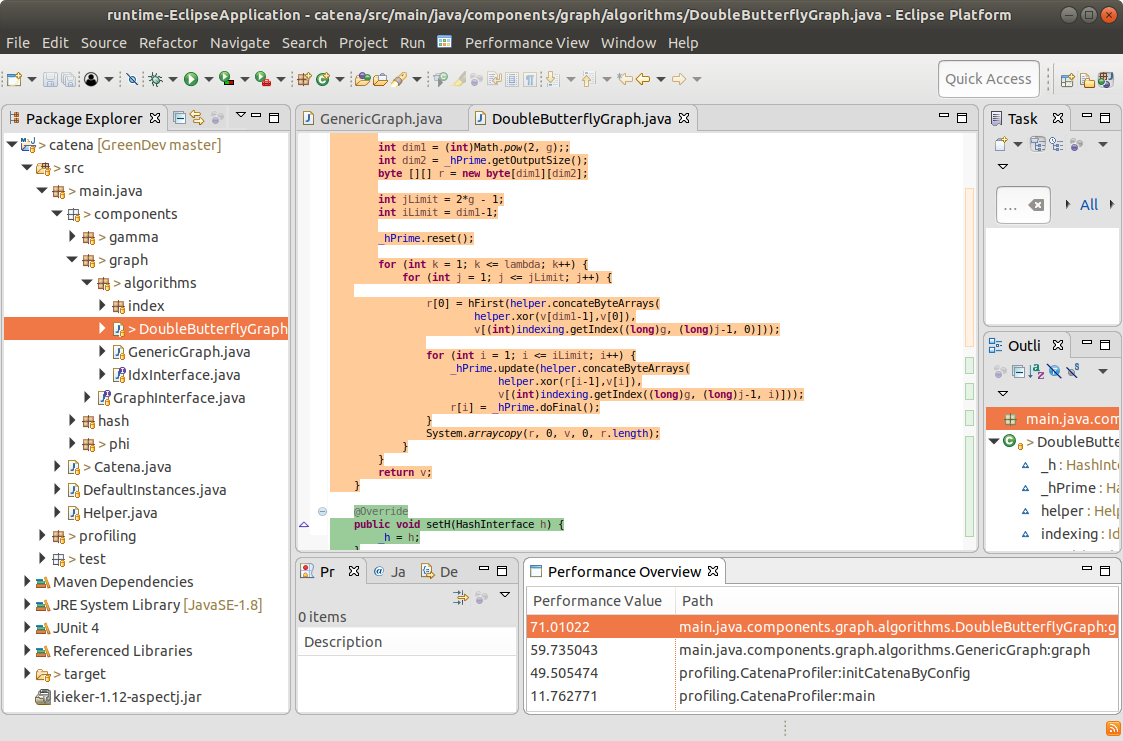
\includegraphics[width=0.8\textwidth]{images/eclipse2}
  \caption{Eclipse Marker Plugin -- Mean over all Configurations.}
  \label{plugin_2}
\end{figure}


The plugin integrated itself into the IDE if the Java perspective is active. It provides a menu for seleting the different modi and an overview area of all colored methodes in the bottom right area of the IDE. In the overview, the methods are sorted in descending order by the performance value. Each line consists of the performance value and the fully qualified name of the method. By double-clicking on a line the corresponding class opens in the main window and scrolls to the clicked method. 


\begin{figure}[h]
  \centering
  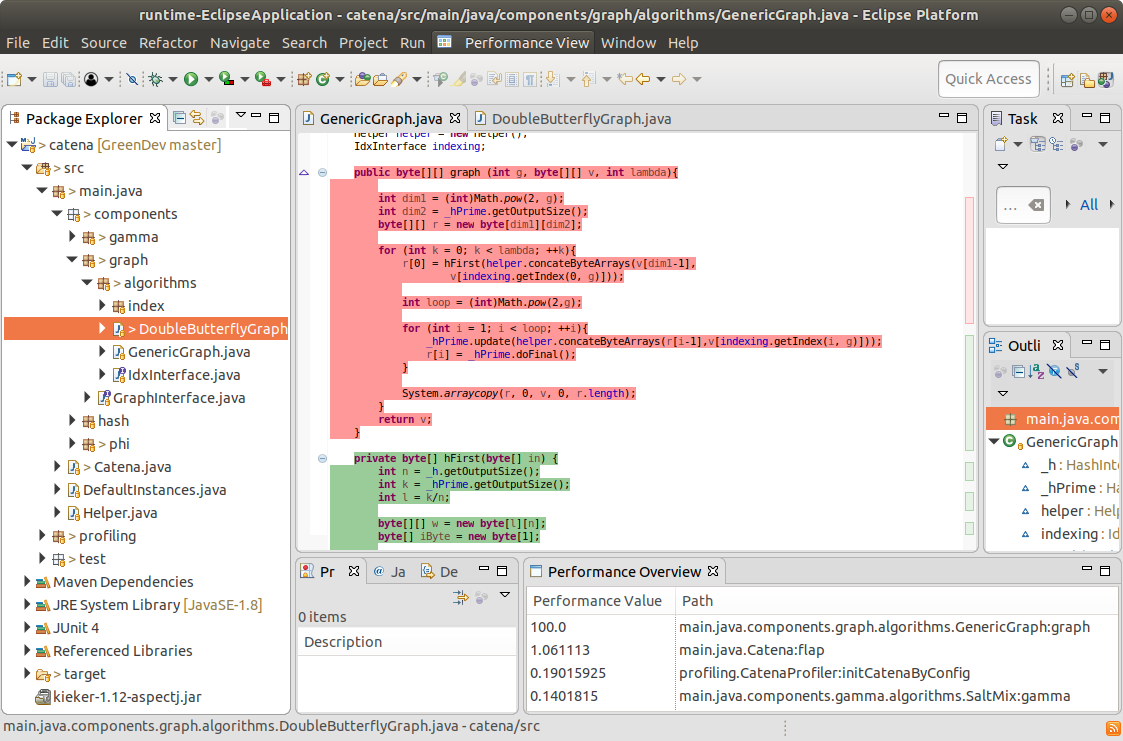
\includegraphics[width=0.8\textwidth]{images/eclipse1}
  \caption{Eclipse Marker Plugin -- Maximum Value over all Configurations.}
  \label{plugin_1}
\end{figure}


Together with a developer of Catena we investigated its performance hot-spots. He confirmed, that there the graphs as well as the flap-method are known as the parts of Catena which consumes most of the performance. 
There are some things still to develop to use this plugin efficiently. Currently it only reads preprocessed data from a database. In the future it would be helpful to automate the process of identifying performance hot-spots with our approach and saving the results such that the plugin can use the information directly. This process needs some manual steps till now.


% structure and functionality (maybe example use case - what is better with this tool in comparison to others)
% discussion of usage scenarios

\subsection{Flame Graphs}
\label{flame_graph}

The second analyse tool we used to present performance of configurable software systems. We used the D3.js plugin\footnote{Available at GitHub: \url{https://github.com/spiermar/d3-flame-graph}.} developed by a Netflix performance engineer. 

\begin{figure}[h]
  \centering
  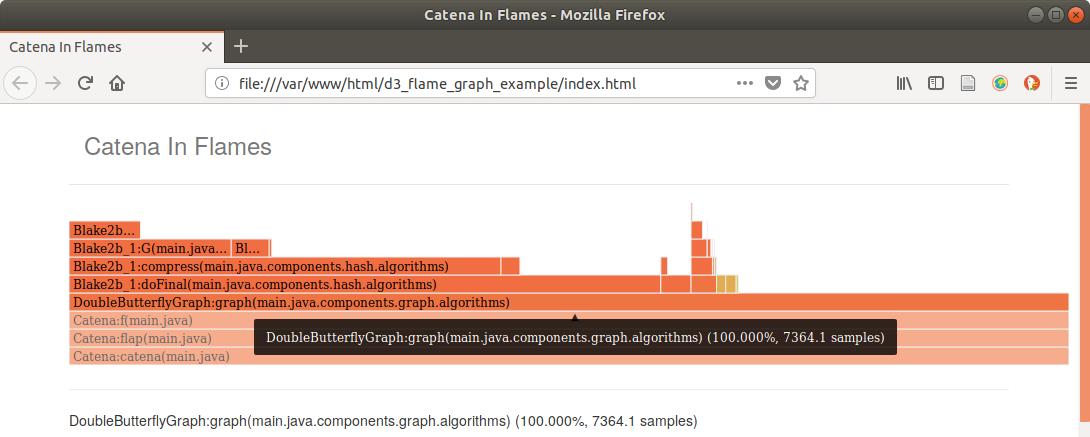
\includegraphics[width=0.99\textwidth]{images/flame_1}
  \caption{Flame Graph -- Catena Performance Visualisation.}
  \label{flame_1}
\end{figure}

In Figure~\ref{flame_1} we show the performance distribution of the methods of one configuration. This example shows the performance of each method of its mean execution time. In this example, we clicked on the DoubleButterflyGraph to zoom in and present the methods performance with the whole width of the visualisation. So we can see, that with this specific configuration the most execution time of Catena is consumed by the DoubleButterflyGraph, but also a lot of performance by the compression() and the doFinal() method of Blake2b\_1. With this visualisation, we have the possibility to investigate all methods in relation the their performance of other methods. 

%Flame graph overview / idea, intention, usage scenario
%discussion of usage scenarios




\section{Threads to Validity}
\label{validity}

In this section we discuss the relevant threads to validity of our approach.


\subsection{Internal Validity}

%Which methodes and analyse metrics


For identifying variants of our subject systems, we used only random sampling in each dimension. Other sampling strategies, specialize to binary or numerical features, lead to another set of samples. It might be that with such strategies, we were able to detect other pattern in the performance data. There are methods in our set of measurements that are biased by more than 20\% by external influences. These methods might introduce a learning bias into our model. In the future, we should analyze the reason for that measurement bias and probably exclude them from our further analysis. The \ac{JIP} measures the execution time of methods with millisecond accuracy. There are profiler like Kieker and SPASSmether that measure within microseconds. This would refine our measurement accuracy by factor 1000. Another thread might be that we only consider pairwise interactions. There are research which proves that there is a number of interactions among three features that influences performance. It might be that this finding also applies on method level. To model different use cases of software, we varied the workloads of our subject systems. But analyzing a databases workload in a real scenario, requires more different workloads and other test scenarios like stress tests or in a client server scenario, other non-functional properties.


\subsection{External Validity}

To achieve a reasonable external validity we used configurable software systems of different application areas (hashing, raytracing, and database) which uses different configuration mechanisms. But to generalize or findings, software systems from other application areas (like flow simulation or even server software) should be analyzed as well. Furthermore, we only used Java-based software systems. It may be that or results are not generalizable to projects that are written in other languages or to commercial software. 

\chapter{Conclusion}
\label{chap:conlusion}

\section{Concluding Remarks}

\section{Outlook and Future Work}


% ---------------------------------------------------------
% References and Appendix
% ---------------------------------------------------------

\bibliographystyle{plain}
\bibliography{bib}
% ---------------------------------------------------------
\chapter*{Acronyms}
% ---------------------------------------------------------

% ---------------------------------------------------------
% Put longest word in square brackets for column spacing
% ---------------------------------------------------------

\begin{acronym}[WWWW]
  \acro{JVM}{Java Virtual Machine}
  \acro{KPI}{Key Performance Indicators}
  \acro{IDE}{Integrated Development Environment}
  \acro{SPL}{Software Product Line}
  \acro{NFR}{Non-functional Requirements}
  \acro{NFP}{Non-functional Properties}
  \acro{SPE}{Software Performance Engineering}
  \acro{CART}{Classification-And-Regression-Tree}
\end{acronym}

\appendix
% ---------------------------------------------------------
\chapter{Appendix}
\label{appendix}
% ---------------------------------------------------------

\section{Feature Diagrams}
\label{feature_diagrams}

\subsection{Running Example}

\lstinputlisting[basicstyle=\scriptsize\ttfamily, captionpos=b, language=xml, caption={Textual representation of example database model.}, label={app_feature_diagrams}]{images/example_database.xml}

\subsection{Case Studies}



% ---------------------------------------------------------
%%\pagestyle{scrheadings}             % Überschriften in den Kopfzeilen
%\tableofcontents
\addcontentsline{toc}{chapter}{\listfigurename}
\listoffigures                      % Abbildungsverzeichnis
\addcontentsline{toc}{chapter}{\listtablename}
\listoftables                       % Tabellenverzeichnis
% \printnomenclature
% \addcontentsline{toc}{chapter}{\nomenclaturename}


\end{document}

